\documentclass[paper=a4, fontsize=11pt]{report}
\usepackage{mathtools}
\usepackage[a4paper,bindingoffset=0.2in,%
            left=1in,right=1in,top=1in,bottom=1in,%
            footskip=.25in]{geometry}


\usepackage{Sweave}
\begin{document}
\Sconcordance{concordance:PreReport.tex:PreReport.Rnw:%
1 7 1 1 0 7 1 1 5 10 1 1 6 1 0 4 1 3 0 1 2 10 1 1 2 16 0 1 2 1 4 3 1 1 %
10 2 0 1 2 4 0 1 5 9 1 1 6 1 0 3 1 3 0 1 5 29 1 1 5 1 3 2 0 2 1 5 0 1 1 %
5 0 1 1 5 0 1 1 6 0 1 2 1 4 15 1 1 7 1 0 3 1 1 2 4 0 1 2 10 1 1 2 1 0 1 %
1 1 2 6 0 1 2 6 0 1 2 13 0 1 5 7 1 1 2 1 0 3 1 6 0 1 2 4 1 1 2 1 0 1 1 %
5 0 1 1 6 0 1 2 1 1 1 2 1 0 1 1 1 2 1 0 1 1 6 0 1 2 1 1 1 70 27 1 1 6 1 %
4 3 0 1 1 3 0 1 2 1 4 15 1 11 0 1 10 3 1 11 0 1 10 2 1 24 0 1 23 7 1 1 %
6 1 7 1 4 9 1 1 6 1 9 1 4 13 1 1 7 1 0 1 1 1 7 6 0 1 1 1 2 1 1 5 0 1 1 %
5 0 1 1 5 0 1 1 6 0 1 5 11 1 12 0 1 11 5 1 14 0 1 13 17 1 14 0 1 13 5 1 %
1 6 1 0 5 1 3 0 1 5 8 1 1 2 20 0 1 18 30 1 1 7 2 0 4 1 5 0 1 1 6 0 1 5 %
11 1 1 2 1 0 3 1 1 2 1 0 3 1 4 0 1 3 11 1 1 3 2 0 1 2 1 0 1 3 2 0 1 2 4 %
0 1 2 2 1 1 3 2 0 1 1 1 2 1 0 1 2 1 0 1 1 3 0 1 2 35 1}

\setlength{\parindent}{0}
\noindent

\title{Emulate \texttt{persp} plot and \texttt{filled.contour} plot on \texttt{gridGraphics}}
\maketitle
\chapter{Introduction}
\section{Background}
The core graphics system in R can been divided in to two main packages. The first package is the graphics package. It is older and it provides the original GRZ graphics system from S, sometimes referred to as ``traditional'' graphics. It is relatively fast and many other R packages build on top of it. The newer package is the grid package. It is actually slower but is has more flexibility and additional features compared to the graphics package. \\

A graph that is drawn using grid can been edited in many more ways than a graph that has been drawn using the basic graphics package. However, there is a new package, called \texttt{gridGraphics}, which allows us to convert a plot that has been drawn by the \texttt{graphics} package to an equivalent plot drawn by \texttt{grid} graphics. This means that the additional flexibility and features of grid become available for any plot drawn using the \texttt{graphics} package. \\

\section{The \texttt{gridGraphics} package}
\texttt{gridGraphics} is like a 'translator' that translates a plot that has been drawn using the basic graphics package to a plot that has been drawn using the grid package. \\

The \texttt{gridGraphic} package has a main function called \texttt{grid.echo()}, which takes a recorded plot as an argument (or NULL for the current plot of the current graphics device). The grid.echo() replicates the plot using grid so that the user may edited the plot in more ways than they can with the original plot drawn by basic graphic package.\\

The following code provides a quick example. We generate 25 random numbers for x and y. First, we draw a scatter plot using the function \texttt{plot()} from the basic graphics package, then we redraw it using \texttt{grid.echo()} from the \texttt{gridGraphics} package with grid.
\begin{Schunk}
\begin{Sinput}
> pdf("figure/report_basic_demo_%0d.pdf", onefile=FALSE)
> dev.control("enable")
> set.seed(110)
> x = runif(25)
> y = runif(25)
> plot(x,y, pch = 16)
> grid.echo()
\end{Sinput}
\end{Schunk}
\newpage
\begin{figure}[h]
\begin{center}
  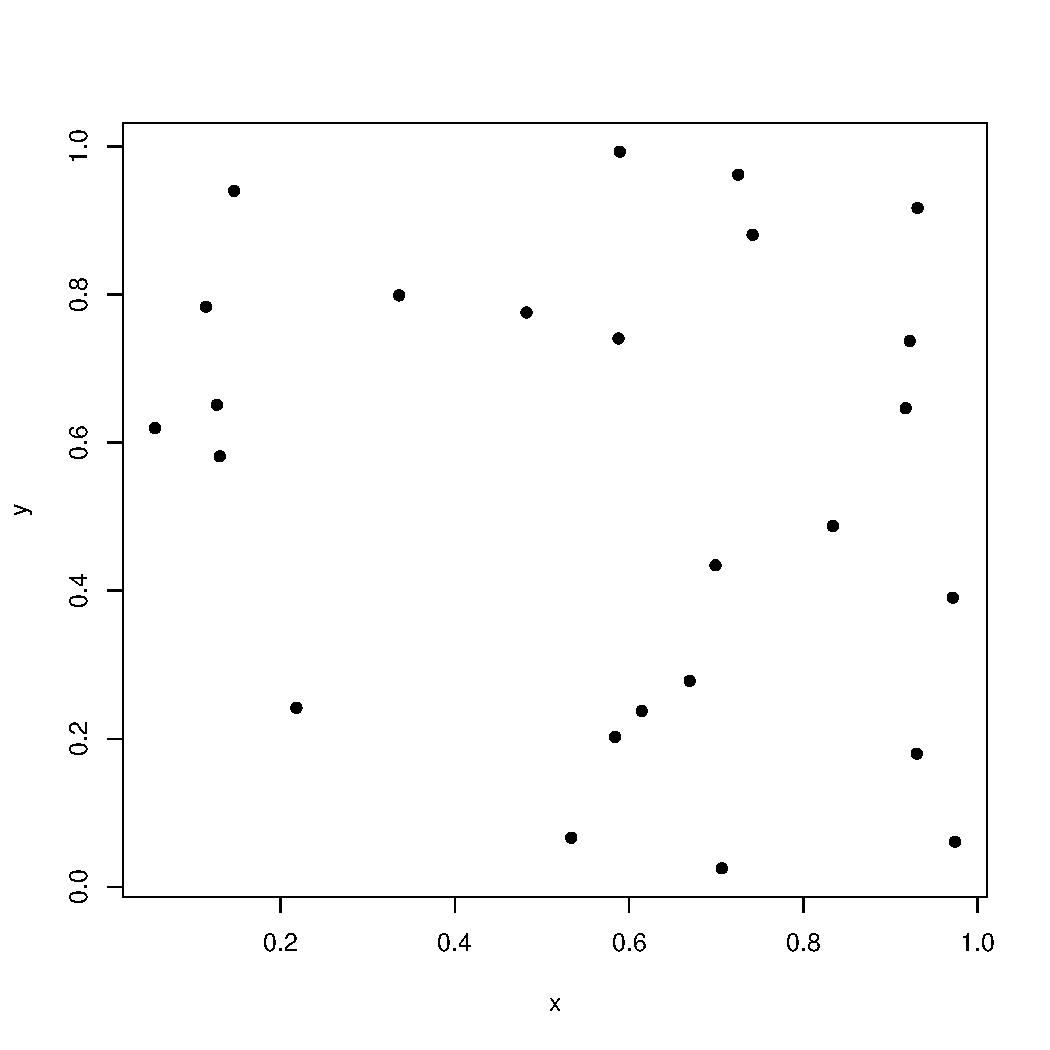
\includegraphics[height = 6cm, width = 6cm]{figure/report_basic_demo_1.pdf}
  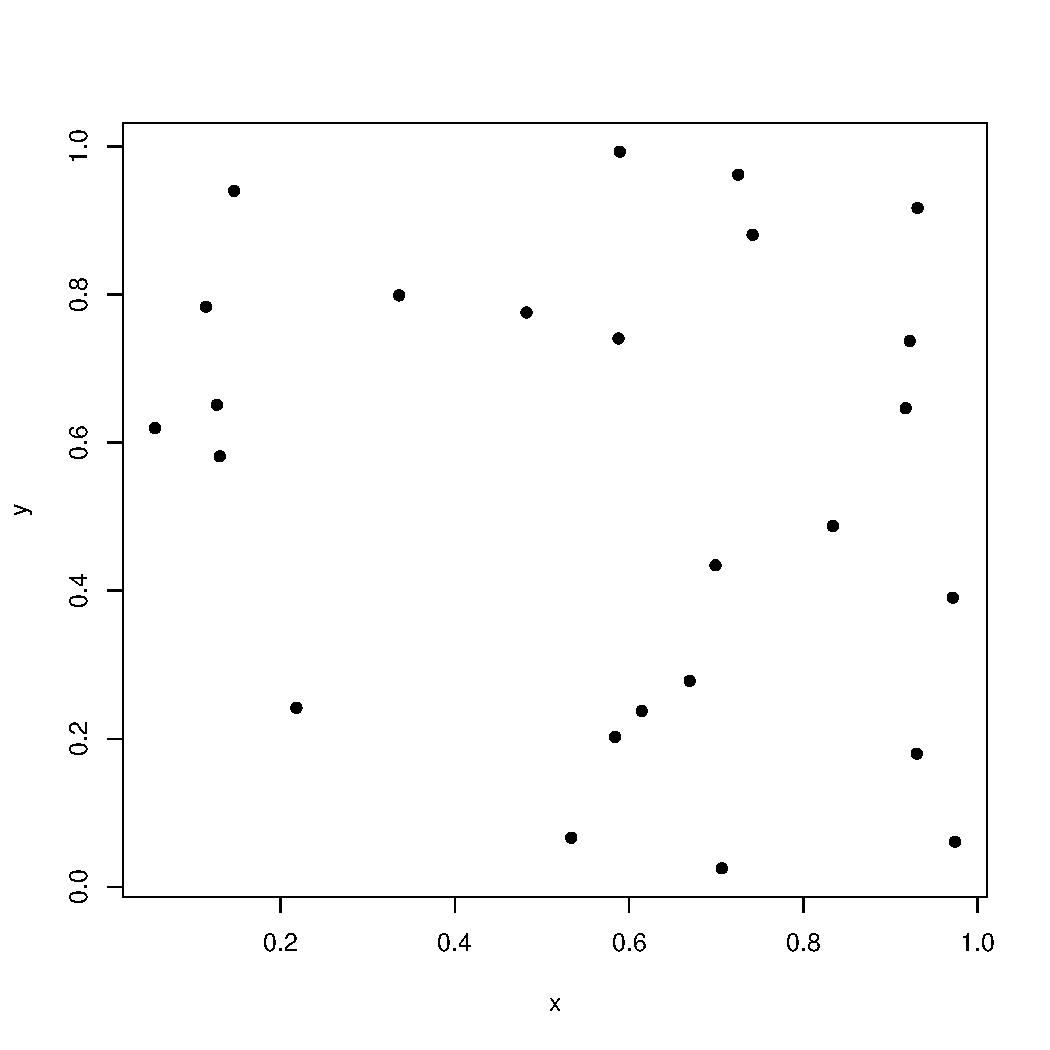
\includegraphics[height = 6cm, width = 6cm]{figure/report_basic_demo_1.pdf}
  \caption{The left plot is drawn by using plot(); the Right plot is redrawn using \texttt{grid.echo()}. Two plots are identical to each other}
  	\label{figure1}
\end{center}
\end{figure}
One example that shows the advantage of drawing the plot using grid rather than basic graphics is that there are objects, called grid grobs, which recorded a list of the details of each components of the plot that has been drawn. The list of grobs can been seen by calling the function \texttt{grid.ls()}. \\
\begin{Schunk}
\begin{Sinput}
> grid.ls()
\end{Sinput}
\begin{Soutput}
graphics-plot-1-points-1
graphics-plot-1-bottom-axis-line-1
graphics-plot-1-bottom-axis-ticks-1
graphics-plot-1-bottom-axis-labels-1
graphics-plot-1-left-axis-line-1
graphics-plot-1-left-axis-ticks-1
graphics-plot-1-left-axis-labels-1
graphics-plot-1-box-1
graphics-plot-1-xlab-1
graphics-plot-1-ylab-1
\end{Soutput}
\end{Schunk}


As we see, the \texttt{grid.ls()} function returns a list of grid grobs for the previous plot that has been redrawn by \texttt{grid}. There is one element called \textit{graphics-plot-1-bottom-axis-labels-1} which represents the labels of the bottom axis. In \texttt{grid}, there are several functions that can be used to manipulate this grob. \\

For example, if the user wants to rotate the labels of the bottom axis by 30 degrees and changes the color from default to orange, then the following code performs these changes.
\begin{Schunk}
\begin{Sinput}
> grid.edit("graphics-plot-1-bottom-axis-labels-1", 
+           rot=30, gp=gpar(col="orange"))
> grid.edit("graphics-plot-1-left-axis-labels-1", 
+           rot=30, gp=gpar(col="orange"))
\end{Sinput}
\end{Schunk}
\begin{figure}[h]
\begin{center}
  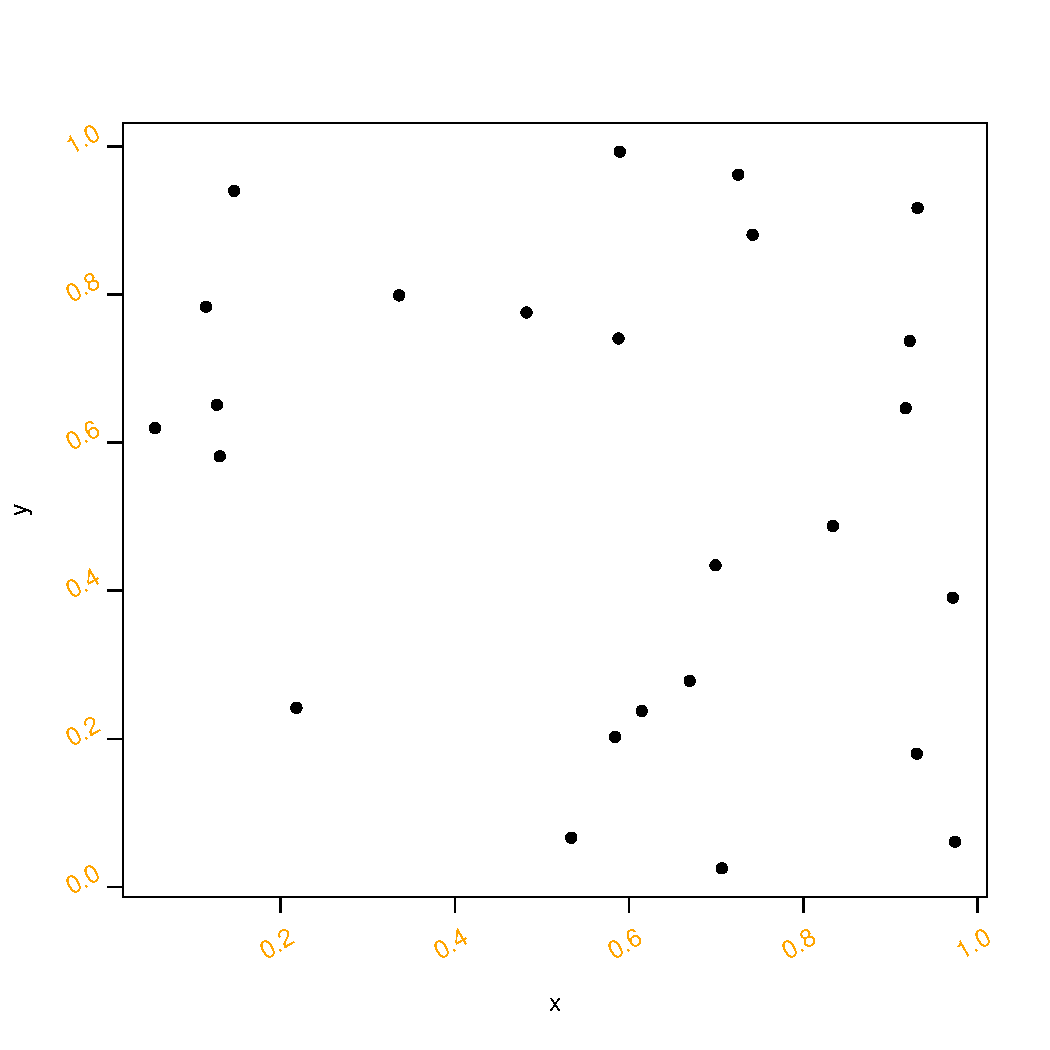
\includegraphics[height = 7cm, width = 7cm]{figure/report_basic_demo_4.pdf}
  \caption{The angle and the color of the bottom and left axis of the previous plot have been changed by 30 degrees and orange}
  	\label{figure3}
\end{center}
\end{figure}
\section{The problem}
The \texttt{grid.echo()} function can replicate most plots that are drawn by the graphics package. However, there are a few functions in the graphics package that \texttt{grid.echo()} cannot replicate. One such function is \texttt{persp()} which draws 3-dimemtional surfaces, the other one is the \texttt{filled.contour()}. If we can draw a plot with \texttt{persp()} or \texttt{filled.countour(),} the result from calling \texttt{grid.echo()} is a (mostly) blank screen. 
\begin{Schunk}
\begin{Sinput}
> x <- y <- seq(-4*pi, 4*pi, len = 27)
> r <- sqrt(outer(x^2, y^2, "+"))
> filled.contour(cos(r^2)*exp(-r/(2*pi)), frame.plot = FALSE, plot.axes = {})
> grid.echo()
\end{Sinput}
\end{Schunk}
\begin{figure}[h]
\begin{center}
  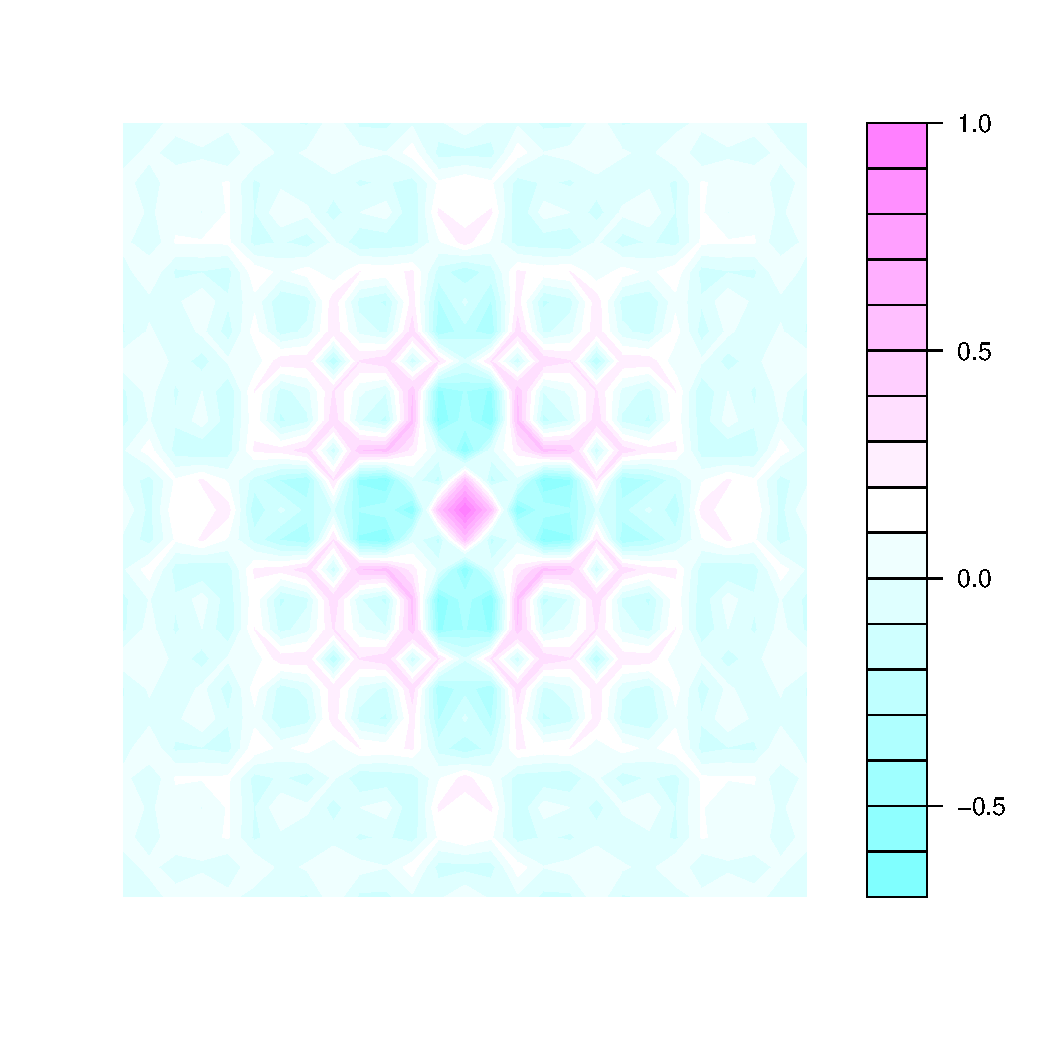
\includegraphics[height = 6cm, width = 6cm]{figure/report_fill_1}
  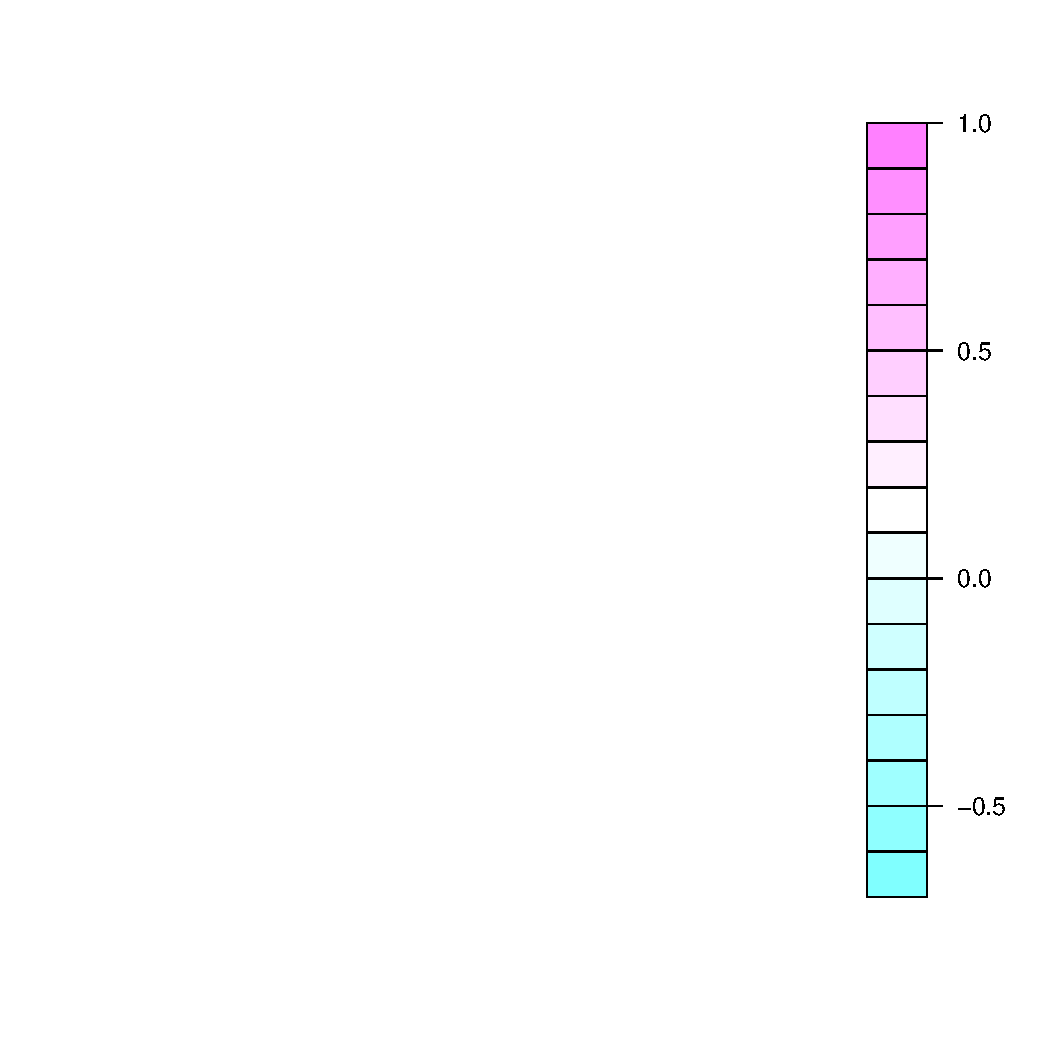
\includegraphics[height = 6cm, width = 6cm]{figure/report_fill_2}
  \caption{The left plot been drawn by using \texttt{filled.contour} and the right plot been redrawn by calling \texttt{grid.echo()}. There is a "blank" page on the right plot because the grid.echo cannot emulate filled.contour()}
  	\label{figure4}
\end{center}
\end{figure}

\section{Aim of this project}
The purpose of this paper is emulate the Perspective Plots, \texttt{persp()} and Level (Contour) Plots, \texttt{filled.contour()} into \texttt{grid} package. However, these two functions are written by C, which is difficult for debugging and tracking. The solution of this paper as follows: 
\begin{enumerate}
  \item Emulate the \texttt{persp()} function on \texttt{grid} separate from the \texttt{gridGraphics} package (standalone):
    \begin{enumerate}
      \item Extract the information from the graphics engine display list.
      \item Understanding and translating the calculation that been done by \texttt{C} code from the \texttt{graphics} package to \texttt{R} code
      \item Draw the Perspective Plot on \texttt{grid}.
    \end{enumerate}
  \item Connect the standalone to the \texttt{gridGraphics}
\end{enumerate}



% NOTE to Jason: explain how gridGraphics works first: graphics display list; gridGraphics implements an R version of each low-level C function on the display list (e.g., for C\_plot\_xy there is an R function called C\_plot\_xy in the gridGraphics package). THEN maybe write about 3D to 2D transformations, but only maybe.% 


\chapter{The graphics engine display list}
The information for every plot drawn by R can be recorded. For example, In the simple \texttt{plot()} function, it is possible to obtain the parameters for x and y, even the label of the x-axis and y-axis.\\

This information is called the graphics engine display list. In this paper, we use this graphics engine display list to replicate the \texttt{persp()} plot and texttt{filled.contour()} plot using grid.\\

The \texttt{recordPlot()} function can be used to access the graphics engine display list, the \texttt{recordPlot()} function been used. This function saves the plot in an R object. 

\begin{Schunk}
\begin{Sinput}
> plot(cars$speed, cars$dist, col = 'orange', 
+       pch = 16, xlab = 'speed', ylab = 'dist')
> reco = recordPlot()[[1]][[4]][[2]][[2]]
> head(reco[[1]]) #x
\end{Sinput}
\begin{Soutput}
[1] 4 4 7 7 8 9
\end{Soutput}
\begin{Sinput}
> head(reco[[2]]) #y
\end{Sinput}
\begin{Soutput}
[1]  2 10  4 22 16 10
\end{Soutput}
\begin{Sinput}
> reco$xlab
\end{Sinput}
\begin{Soutput}
[1] "cars$speed"
\end{Soutput}
\begin{Sinput}
> reco$ylab
\end{Sinput}
\begin{Soutput}
[1] "cars$dist"
\end{Soutput}
\end{Schunk}


\begin{figure}[h]
\begin{center}
  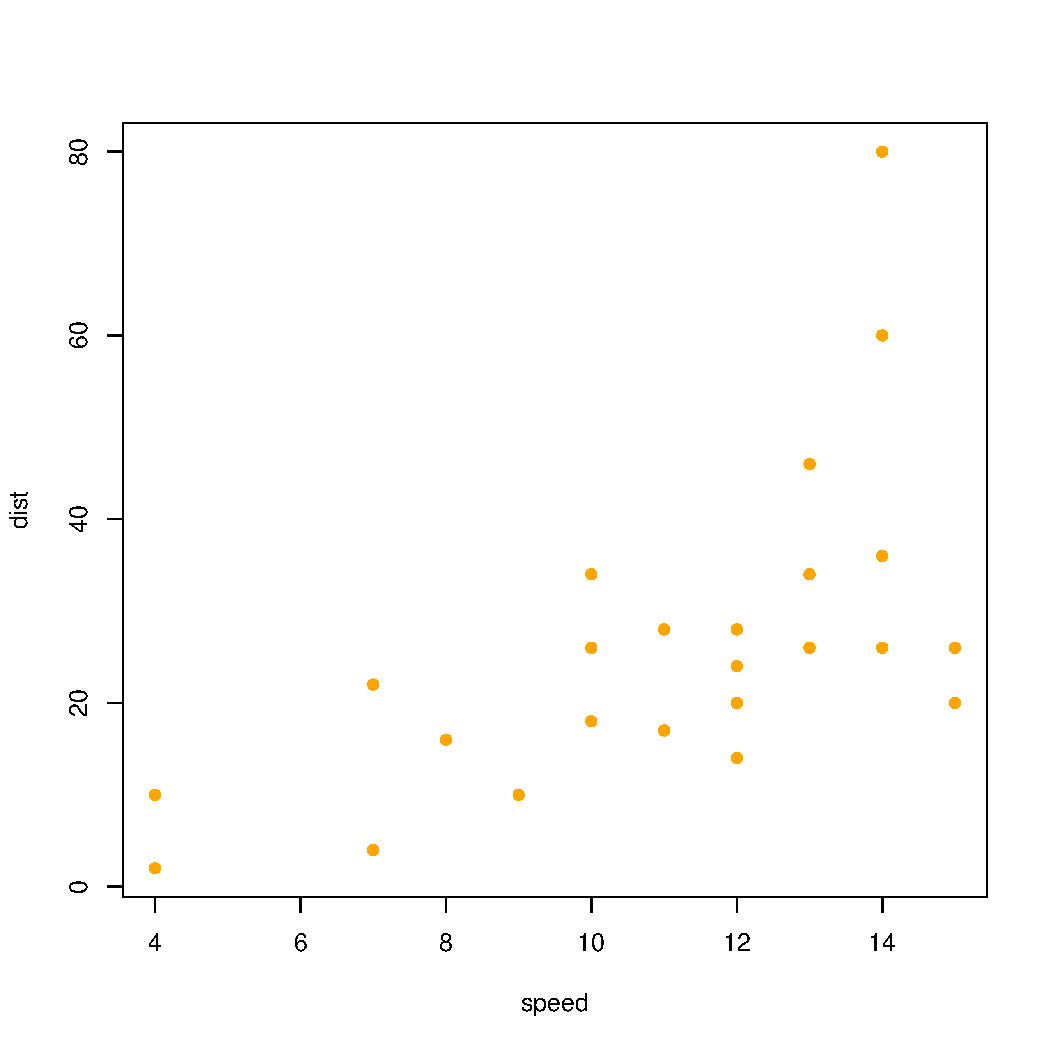
\includegraphics[height = 8cm, width = 8cm]{figure/report_3.pdf}
  \caption{The details of the plot of dist vs speed displayed by the graphics engine display list}
  	\label{figure4}
\end{center}
\end{figure}

The example demonstrates how to access the graphics engine display list of a plot drawn by \texttt{plot}. The values of x and y, the labels of x-axis and y-axis been displayed.



\chapter{Standalone}
\section{The Perspective Plots \texttt{persp()}}
The Perspective Plots \texttt{persp()} is used to draw a surface over the x-y plane. Usually, it has three main argument, \textbf{x, y, z}. Where \textbf{x} and \textbf{y} are the locations of grid line which the value z been measured, \textbf{z} is a matrix which containing the values that been used to plot, or it is the matrix that been calculated by a specific function, such as 3-D mathematical functions. The following example shows how to draw a obligatory mathematical surface rotated sinc function on Perspective Plot.
\begin{Schunk}
\begin{Sinput}
> x = y = seq(-10, 10, length= 60)
> f <- function(x, y) { r <- sqrt(x^2+y^2); 10 * sin(r)/r }
> z <- outer(x, y, f)
> z[is.na(z)] <- 1
> trans = persp(x, y, z, theta=30, phi = 20, expand = 0.5,
+               col = 'White', border = 'orange')
\end{Sinput}
\end{Schunk}
\begin{figure}[h]
\begin{center}
  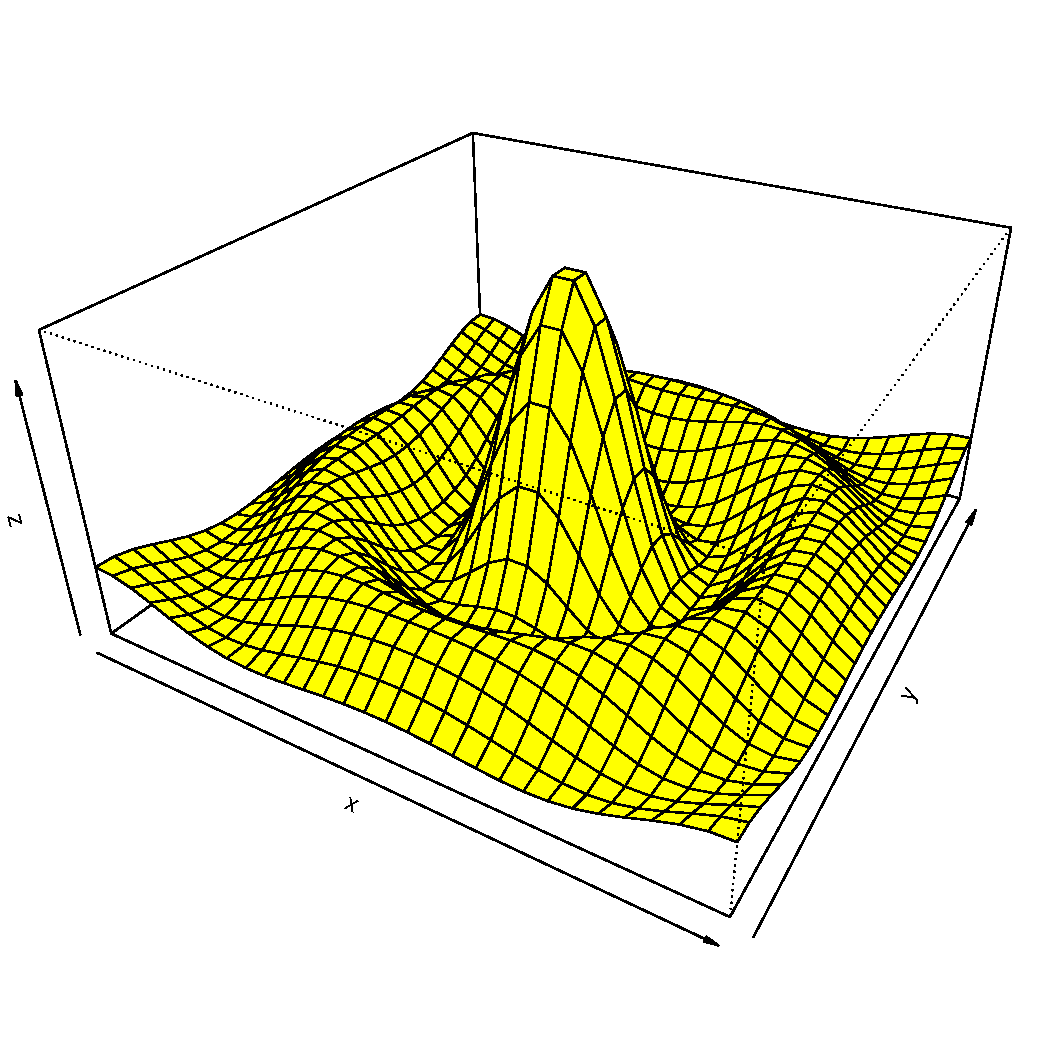
\includegraphics[height = 7cm, width = 7cm]{figure/standalone_1.pdf}
  \caption{An example of Perspective Plot been drawn by \texttt{persp()}}
  	\label{figure4}
\end{center}
\end{figure}

From the previous example, it is clearly to see that the Perspective Plots is formed by a finite number of "polygon", each polygon has 4 Vertices. If we can access the values for each Vertices of the polygon, then we can reproduce this polygon. If we can access all the values of Vertices of all polygons, then we can reproduce the Perspective Plot. \\

Inorder to emulate this plot, we need to access some information from the graphics engine display list. However, the value of the vertices is not in the display list, therefore the plot cannot be reproduced directly. But we can access value of \textbf{x}, \textbf{y} and \textbf{z}, therefore we should re-do the calculation to get values of all vertices. The following codes show that the value of \textbf{x}, \textbf{y} and \textbf{z} which inputted by the user can been "catched" from the display list.
\begin{Schunk}
\begin{Sinput}
> reco = recordPlot()
> info = reco[[1]][[3]][[2]]
> ## print the values of x
> head(info[[2]])
\end{Sinput}
\begin{Soutput}
[1] -10.000000  -9.661017  -9.322034  -8.983051  -8.644068  -8.305085
\end{Soutput}
\begin{Sinput}
> ## print the values of y
> head(info[[3]])
\end{Sinput}
\begin{Soutput}
[1] -10.000000  -9.661017  -9.322034  -8.983051  -8.644068  -8.305085
\end{Soutput}
\begin{Sinput}
> ## print the values of z
> info[[4]][1:6, 1:2]
\end{Sinput}
\begin{Soutput}
          [,1]      [,2]
[1,] 0.7070981 0.6998135
[2,] 0.6998135 0.6510811
[3,] 0.6534671 0.5639162
[4,] 0.5714305 0.4439461
[5,] 0.4589249 0.2984302
[6,] 0.3225432 0.1356653
\end{Soutput}
\end{Schunk}
\subsection{The translation from 3-D points into 2-D points}
The values of \textbf{x}, \textbf{y} and \textbf{z} can been recored from the display list, which been explained by the pervious section, the next task is to use this information to reproduce the vertics in 3-D.\\

As we know, the matrix, \textbf{z} is computed by a specific functions, given two inputs, \textbf{x} and \textbf{y}, or the expression of z can been written as: $z = f(x,y)$, it contains all the values for all combination of \empth{x} and \textbf{y} and the dimenstion of \textbf{z} is $ \textbf{dim(x)} \times \textbf{dim(y)}$.\\

One 3-dimenstions points contains a set values of $(x, y, z)$, but \textbf{z} is $\textbf{dim(x)} \times \textbf{dim(y)}$ matrix, \textbf{x} is a vector which has length of $\textbf{length(x)}$ and \textbf{y} is a vector which has length of $\textbf{length(y)}$. Inorder to produce the points, the D of \textbf{x}, \textbf{y} and \textbf{z} need to be matched and in a right order.\\

First step is the reduce the \textbf{z} $\textbf{dim(x)} \times \textbf{dim(y)}$ matrix into a one D vector which has length of $\textbf{dim(x)} \times \textbf{dim(y)}$. It can be reduced by either along x direction or y direction. In this paper, we reduced along the x direction. The second step is repeat the vector x and y until the same length of \textbf{z}. Since \textbf{z} is reduced along the x direction say $z_p$, hence we repeat x until the length of y say $x_p$, and we repeat each y by the length of \textbf{x}, say $y_p$. At last, the combination of $\x_p$, $y_p$, $z_p$ is the 3-D points which prepare for computing the vertices. \\
\begin{Schunk}
\begin{Sinput}
> xTmp = rep(x, length(y))
> yTmp = rep(y,each = length(x))
> zTmp = as.numeric(z)
> length(xTmp) == length(zTmp) & length(yTmp) == length(zTmp)
\end{Sinput}
\begin{Soutput}
[1] TRUE
\end{Soutput}
\end{Schunk}

The idea of transform the points into vertices is repeating the points in a right order. From pervious section, we explained that the Perspective Plots is made by finite number of polygons. Each polygon has 4 vertices. The total number of polygons are required to be drawn is depend on the length of input \textbf{x} and the length of input \textbf{y}, that is, \textbf{total = (length(x) - 1) $\times$ (length(y) - 1)}. The polygons been drawn by connecting 4 points in a specific order. The algorithm of the drawing as follows: starting from bottom-left, first connect bottom-left to bottom-right, second connect from bottom-rigth to top-right, lastly, connect top-right to top-left. Every polygon is being drawn in this order. The surface of Perspective Plots is formed until all the polygons are been drawn. \\

Before drawing the surface, the transformation of 3-D vertices into 2-D vertices is required. This transformation required two main variables, the 3-D vertices and $4 \times 4$ viewing transformation matrix \textbf{P}. The 3-dimenstion vertices are computed, the matrix \textbf{P} can been recored from the \texttt{persp()} call. This transformation can be done easily on R by using the \texttt{trans3d()} function.

\begin{Schunk}
\begin{Sinput}
> points3d = trans3d(xTmp, yTmp, zTmp, trans)
> head(points3d$x)
\end{Sinput}
\begin{Soutput}
[1] -0.3928108 -0.3861145 -0.3792354 -0.3721881 -0.3649927 -0.3576724
\end{Soutput}
\begin{Sinput}
> head(points3d$y)
\end{Sinput}
\begin{Soutput}
[1] -0.1066821 -0.1090048 -0.1121947 -0.1161865 -0.1208728 -0.1261142
\end{Soutput}
\end{Schunk}

Because of we are drawing a 3-D surface in a 2-D plane, some polygons that stay 'behind' cannot been seen, it is necessary to draw the polygons in a right order. The order defined by using the \textbf{x} and \textbf{y} coordinate of the 3-D vertices (but ignore the \textbf{z} coordinate) combinding another column \textbf{1}, then do the matrix multiplication with the viewing transformation \textbf{P}. The fourth column from this multiplication is the drawing order of the polygons.
\begin{Schunk}
\begin{Sinput}
> orderTemp = cbind(xTmp, yTmp, 0, 1) %*% trans 
> zdepth = orderTemp[, 4]
> ## the zdepth of a set of 4 points of each polygon
> a = order(zdepth, decreasing = TRUE)
> head(a)
\end{Sinput}
\begin{Soutput}
[1] 3541 3542 3481 3543 3482 3544
\end{Soutput}
\end{Schunk}

The following figures shows how does this paper approximate to the solution. The top-left figure is drawn by plotting the transformed 2-dimenstion points, the shape of the Perspective Plots been presented. The top-right figure is drawn by connecting the points line-by-line, the shape become more obvious. The bottom-left figure is drawn by using the \texttt{grid.polygon()}. By default, the origin order of the polygons is drawn along x-axis, then along y-axis. Clearly this is not the correct order. Finally, the bottom-right figure shows the true Perspective Plots by fixing the order. 
\newpage
\begin{figure}[h]
\begin{center}
  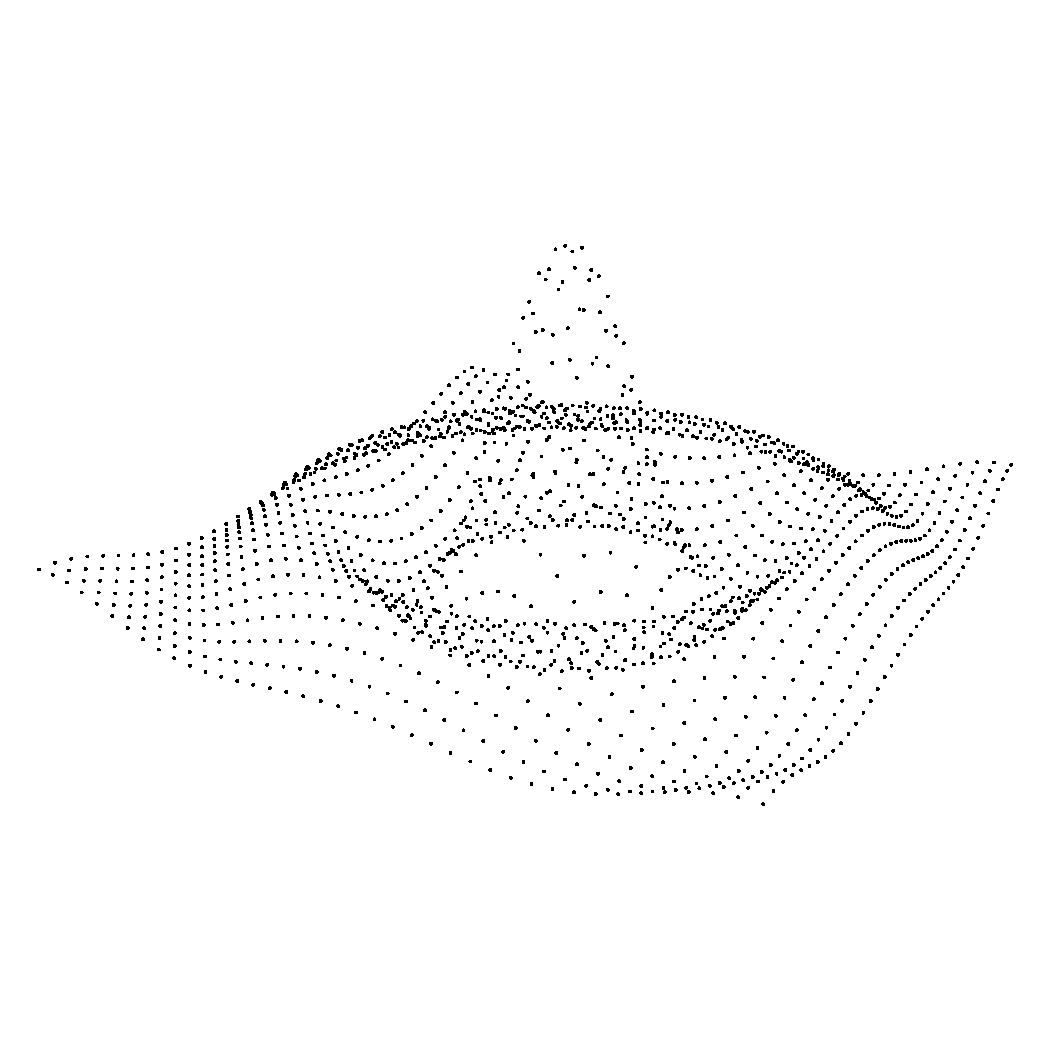
\includegraphics[height = 6cm, width = 6cm]{figure/standalone_p_1.pdf}
  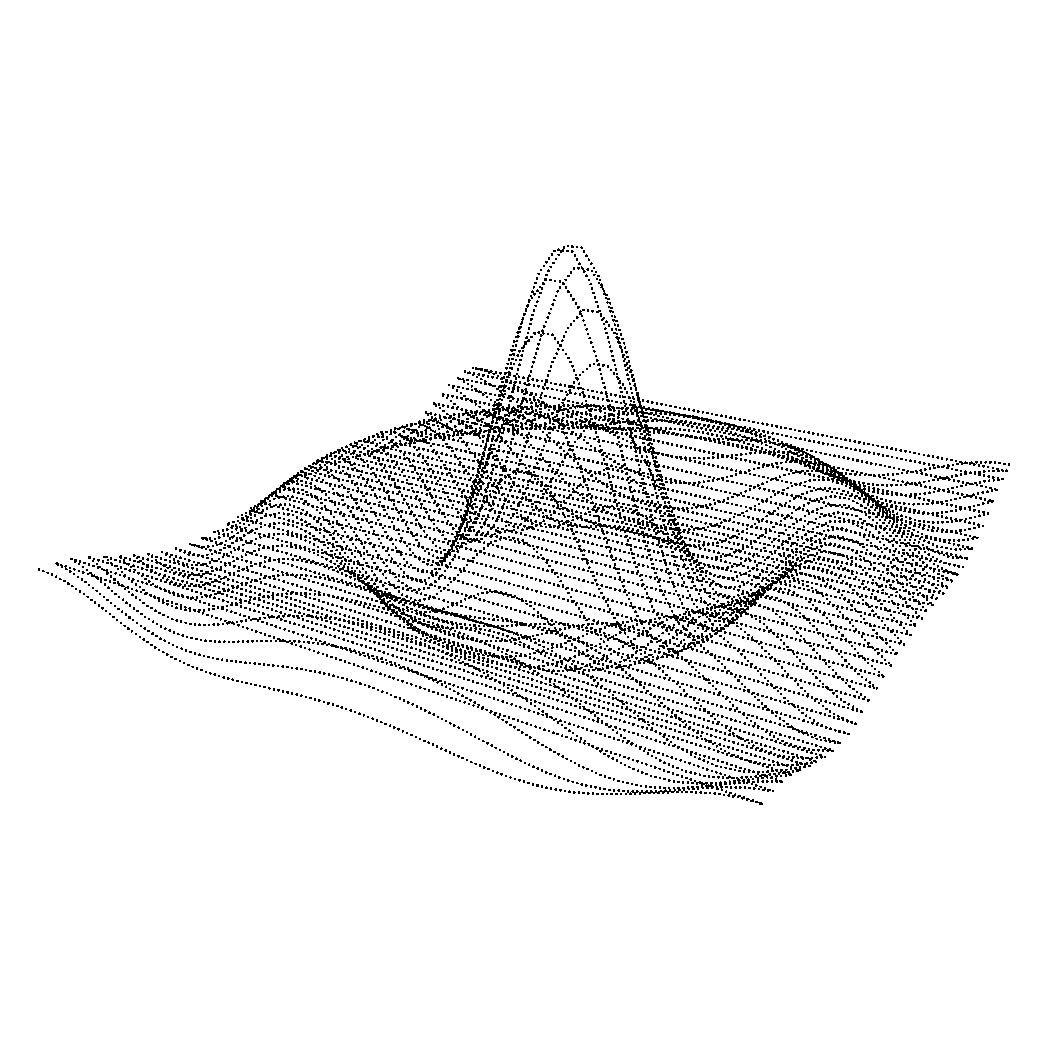
\includegraphics[height = 6cm, width = 6cm]{figure/standalone_p_2.pdf}
  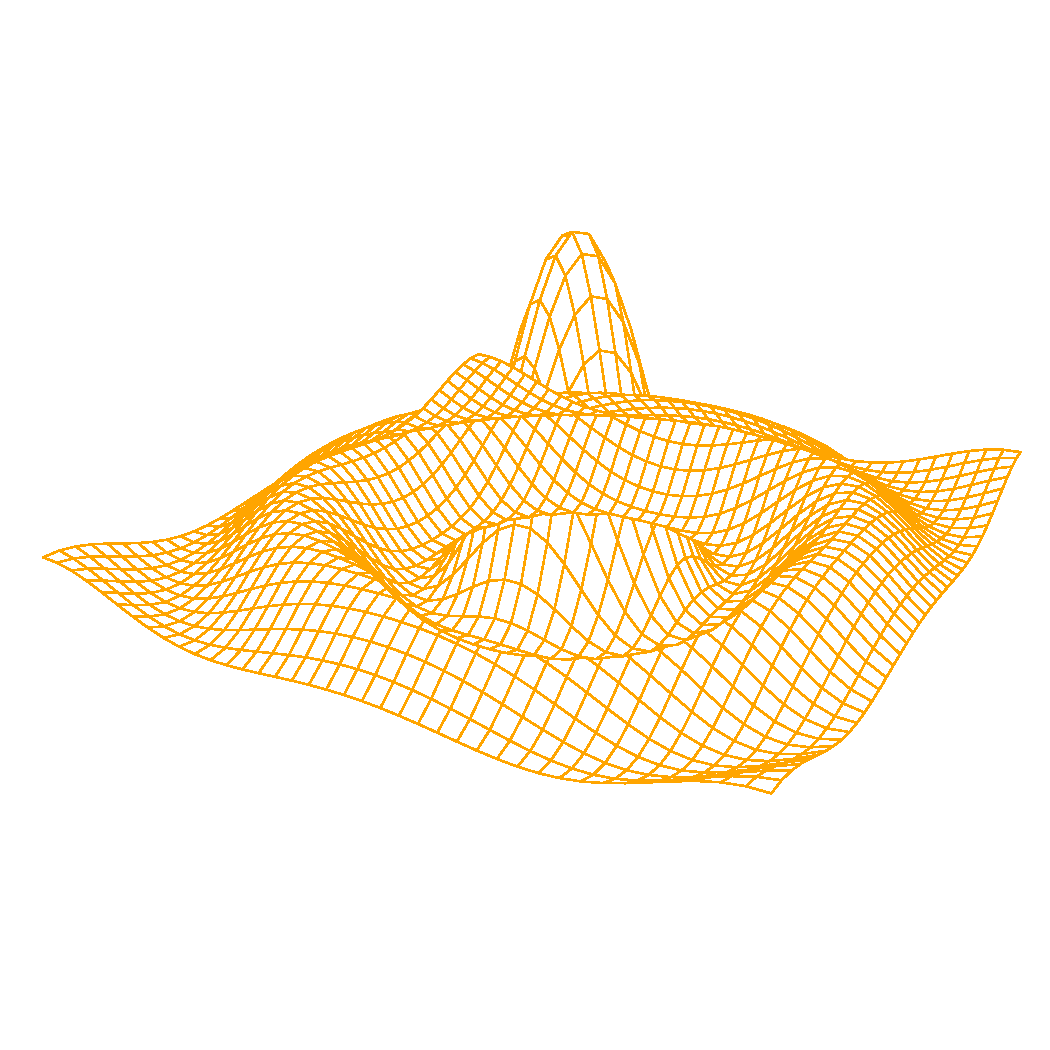
\includegraphics[height = 6cm, width = 6cm]{figure/standalone_p_3.pdf}
  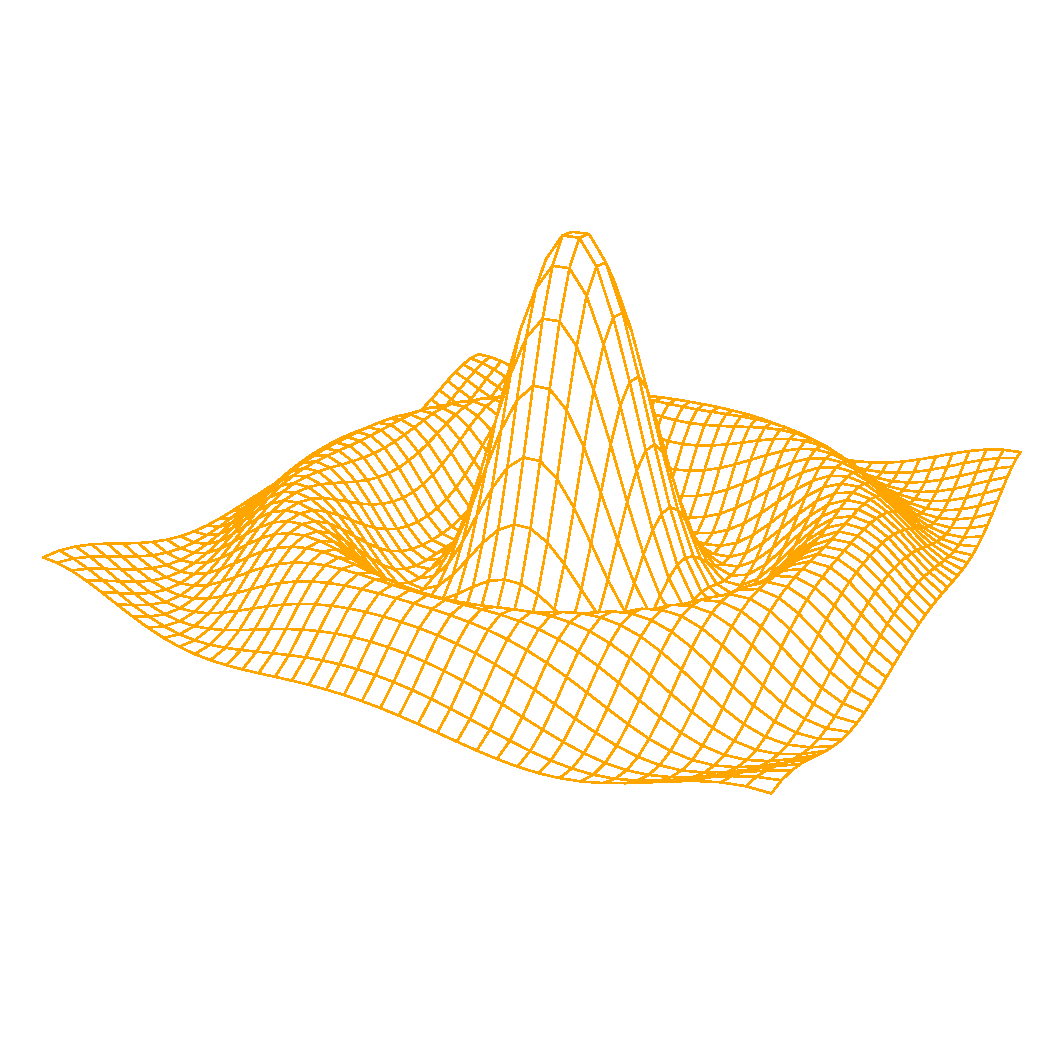
\includegraphics[height = 6cm, width = 6cm]{figure/standalone_p_4.pdf}
  \caption{The top-left figure is only plotting the transformed 2-dimenstion points. The top-right figure is being drawn by connecting the points line-by-line. The top-right figure is drawn unorderly by using the \testtt{grid.polygon}. Finally, the bottom-left figure is drawn in a correct order.}
  	\label{figure4}
\end{center}
\end{figure}

\subsection{Lighting}
The other main benifit supported by \texttt{persp()} is the shadding. It shades the surface by assuming the surface being illuminate from a given direction.(light source)\\

In \texttt{persp()}, the main parameters that user need to specify for produce a shaded perspective plots are: \textit{ltheta}, \textit{lphi} and \textit{shade}.\\

\textit{ltheta} and \textit{lphi} are used for setting up the direction of the light source. In particular, \textit{ltheta} specified the angle in z direction, \textit{lphi} specified the angle in x direction. \\

\textit{shade} is the parameter that specified the shade at each facets of the surface, the shades will compute as follows:
\begin{equation}
\big(\frac{1 + d}{2}\big)^{shade}
\end{equation}
Where \textit{d} is the dot product of the unit vector normal to each of the facet(\textit{u}) and the unit vector of the direction of the light(\textit{v}). \\

The color of each facet will be calculated by the color that recored from the graphics engine display list multiply by the \textbf{shade}. Finally, the surface been drawn by filling the colors for every facet.\\

If the normal vector is perpendicular to the direction of the light source, then $d = 0$ and the term $\big(\frac{1 + d}{2}\big)^{shade}$ will be close to 0, therefore the corrosponding facets will become darker, the brightness and darkness will depend on the value of the \textbf{shade} if shade close to 0, the term $\big(\frac{1 + d}{2}\big)^{shade}$ will close to 1. Therefore, it will look similar to non-shading plot. Simiarlly, if shade gets larger, the term close to 0 and the plot gets darker.

\begin{Schunk}
\begin{Sinput}
> trans = persp(x, y, z, theta=30, phi = 20, expand = 0.5,
+  col = 'White', border = 'NA', shade = 0.5, ltheta = 30, lphi = 20)
> grid.echo()
\end{Sinput}
\end{Schunk}


\begin{figure}[h]
\begin{center}
  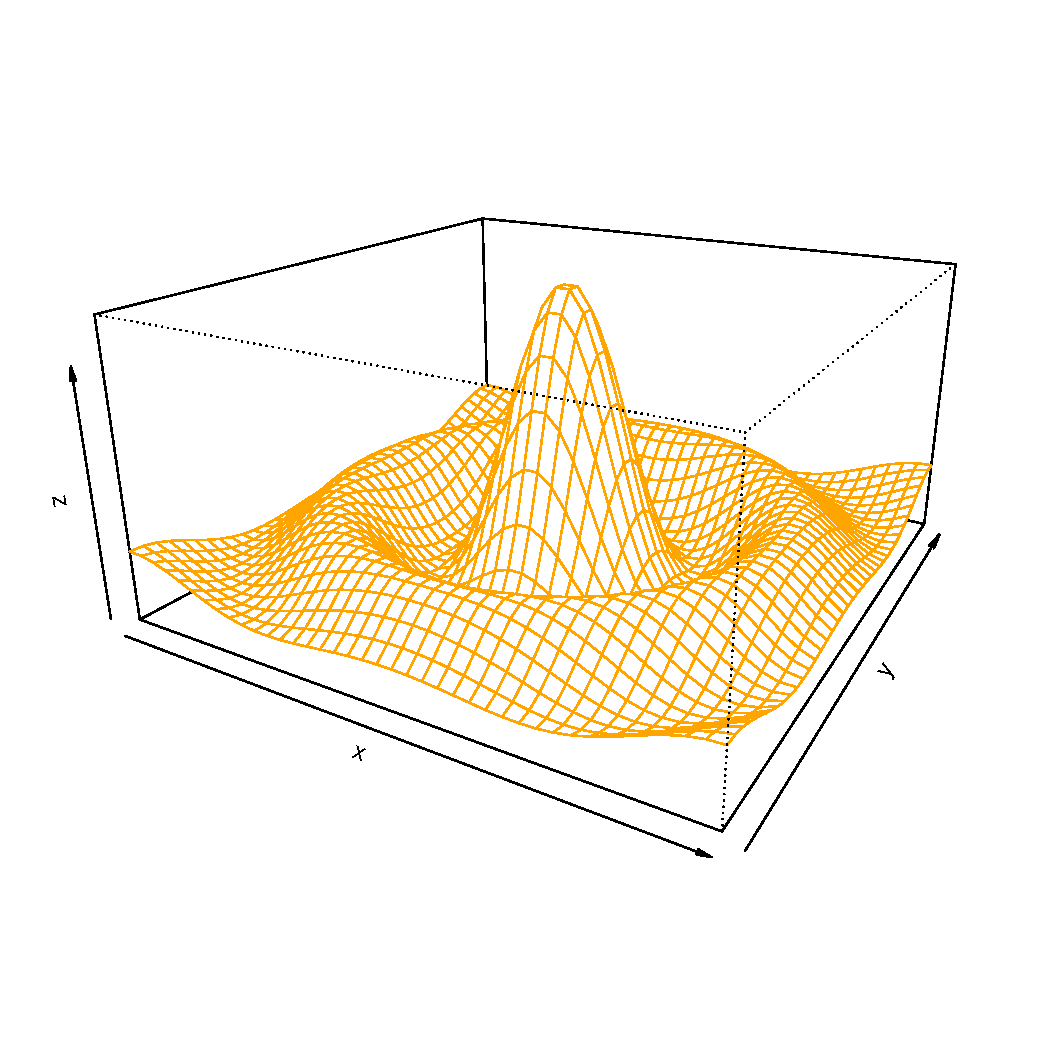
\includegraphics[height = 6cm, width = 6cm]{figure/Lighting_1.pdf}
  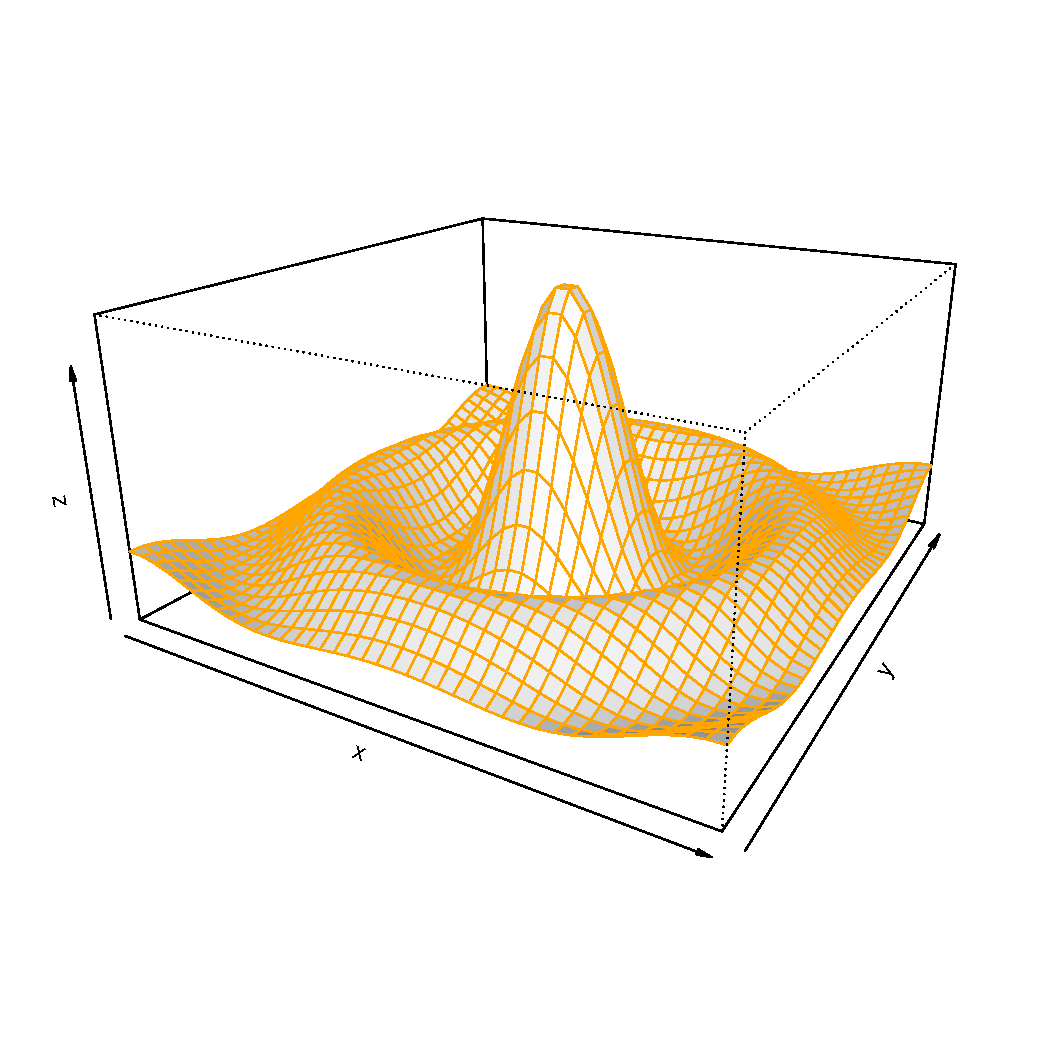
\includegraphics[height = 6cm, width = 6cm]{figure/Lighting_2.pdf}
  \caption{Adding a light source to the perspective plot from the same angel of view. The left figure been drawn by \texttt{graphics} and the right figure been drawn by \texttt{grid}, they are identical to each other.}
  	\label{figure7}
\end{center}
\end{figure}

\subsection{Difference beween \texttt{C} and \texttt{R}}
As we know, most base functions of \texttt{R} are been written by \texttt{C} include \texttt{persp} and \texttt{fill.contour}. Although the structure of \texttt{C} code is quite similar to \texttt{R} code in some special case, there are some \texttt{C} code structures which behave completely different to \texttt{R}, therefore translate \texttt{C} code to \texttt{R} code is not just "copy-and-paste", even just doing direct translation.\\

\subsubsection{Pointers}
One main data structure in \texttt{C} is the pointers, which is a type of reference that records the address/location of a global object or a local variable in a function. Pointers can be manipulated by using assignment or pointer arithmetic.
\begin{Schunk}
\begin{Sinput}
> # static int LimitCheck(double *lim, double *c, double *s)
> # {
> #     if (!R_FINITE(lim[0]) || !R_FINITE(lim[1]) || lim[0] >= lim[1])
> # 	return 0;
> #     *s = 0.5 * fabs(lim[1] - lim[0]);
> #     *c = 0.5 * (lim[1] + lim[0]);
> #     return 1;
> # }
\end{Sinput}
\end{Schunk}
The top piece of code is used for checking the Limit for the \texttt{persp()} function. It also multifying the variable \textttt{c} and \texttt{s} for further calculation. In this case, the \texttt{*c} and \texttt{s*} are the pointer which will pointing to the mechine memory of \texttt{s} and \texttt{c} and multify them.\\

However, this process cannot be reproduced on \texttt{R} because \texttt{R} does not have the pointer data structure. One possible solution will be rather than doing the Limit checking and multify \texttt{s} and \texttt{c}, do the limit checking and return/assign the \texttt{s} and \texttt{c} as xs ad ys for further calculation.
\begin{Schunk}
\begin{Sinput}
> # LimitCheck = function ( lim ) {
> #     ## not finished yet...
> #     s = 0.5 * abs(lim[2] - lim[1])
> #     c = 0.5 * (lim[2] + lim[1])
> #     c(s, c)
> # }
> # xs = LimitCheck(xr)[1]
> # xc = LimitCheck(xr)[2]
> # ...
\end{Sinput}
\end{Schunk}
\subsubsection{Array}
The other main difference is that \texttt{C} use array data format rather than matrix data format in \texttt{R}. However, the indexing of elements in matrix is identical to the indexing of elements in array. 
\begin{Schunk}
\begin{Sinput}
> #...
> 
> # FindPolygonVertices(c[k - 1], c[k],
> #         x[i - 1], x[i],
> #         y[j - 1], y[j],
> #         z[i - 1 + (j - 1) * nx],
> #         z[i + (j - 1) * nx],
> #         z[i - 1 + j * nx],
> #         z[i + j * nx],
> #         px, py, pz, &npt);
> 	    
> 
> #out = FindPolygonVertices(sc[k], sc[k + 1],
> #        x[i], x[i + 1],
> #        y[j], y[j + 1],
> #        z[i + (j - 1) * nx],
> #        z[i + 1 + (j - 1) * nx],
> #        z[i + (j) * nx],
> #        z[i + 1 + (j) * nx],
> #        px, py, pz, npt, iii = iii)
> #...
\end{Sinput}
\end{Schunk}
To get the "same" elements in the matrix as the elements in the array, one solution will be that changing the matrix data format into vector data format, so that the elements will be stay the same location for both array, and matrix data format.\\

The top piece of codes is both calling the \texttt{FindPolygonVertices()} function by feeding parameter into it. However, the \texttt{z} is array in the first call as it written on \texttt{C} but the second is matrix as it written on \texttt{R}. the - 1 on the \texttt{R} code because \texttt{C} starting at 0 index but \texttt{R} starting at 1.\\

\subsection{Box and other features}
One feather that \texttt{persp()} supported is whether draw a container (box) around the surface. In Figure 5, both surface and box been drawn in the plot. However, it is necessary to find out whether the edge of the box in front of the surface or behind the surface. \\

The solution will be that translates the \texttt{C} code to \texttt{R} code directly. The reason for doing this directly translation is that R is sensitive on drawing the dot lines. More specifically, it may cause difference if we connect two points with a dotted line in different direction. Due to the purpose of this paper, the plot should be drawn as identical as possible. Therefore, the direct translation is required.\\


\newpage
\begin{figure}[h]
\begin{center}
  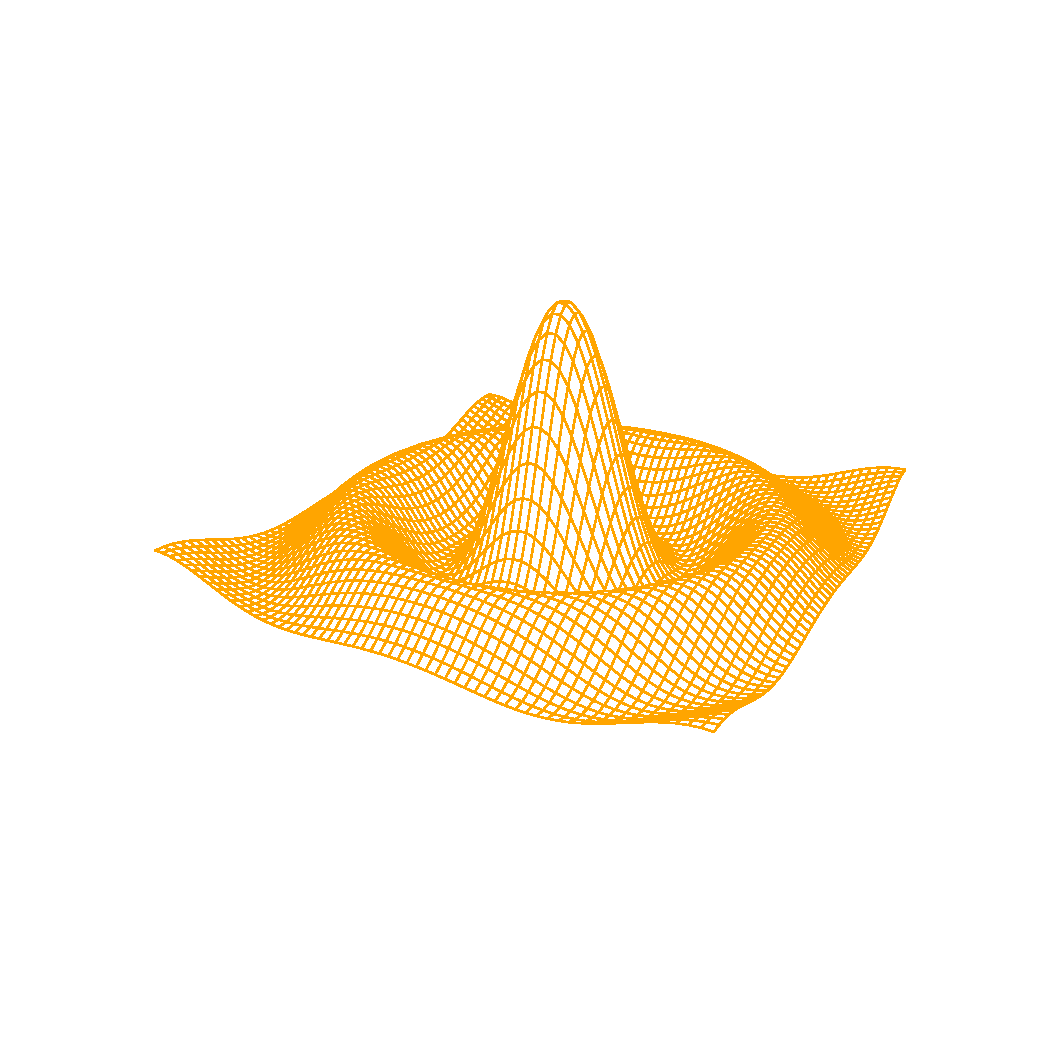
\includegraphics[height = 6cm, width = 6cm]{figure/box_example_1.pdf}
  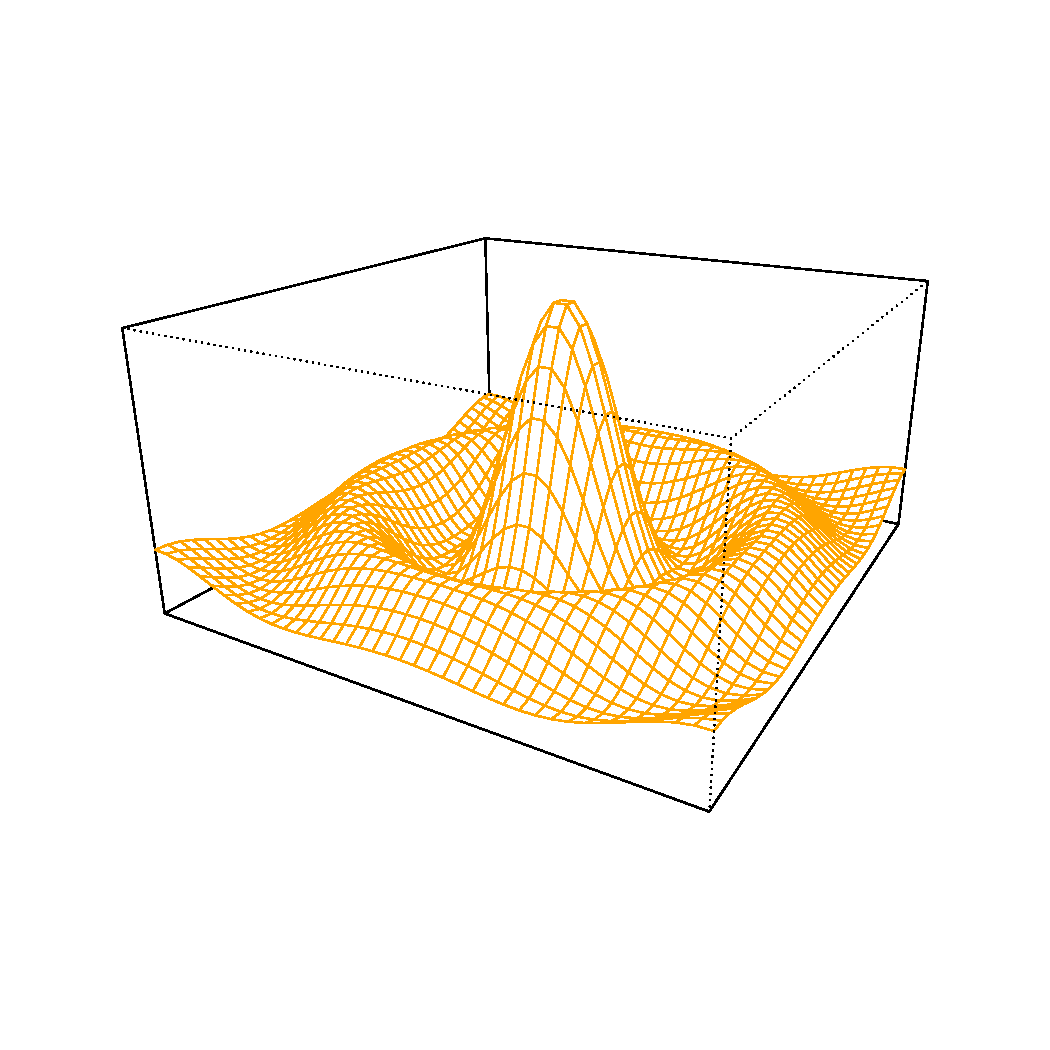
\includegraphics[height = 6cm, width = 6cm]{figure/box_example_2.pdf}
  \caption{The surace been drawn by ignore the box in the left plot, right plot drawn the surface as well as box}
  	\label{figure8}
\end{center}
\end{figure}

Other feather that \texttt{persp} supported is the detail of the axis. More specifily, the axis has three type, no axes, simple axes which only contain the label of axes, or showing the scale of each axes. These feathers are required to be reproduced by \texttt{grid}, The solution to this problem by translating the \texttt{C} code to \texttt{R} code directly.



\begin{figure}[h]
\begin{center}
  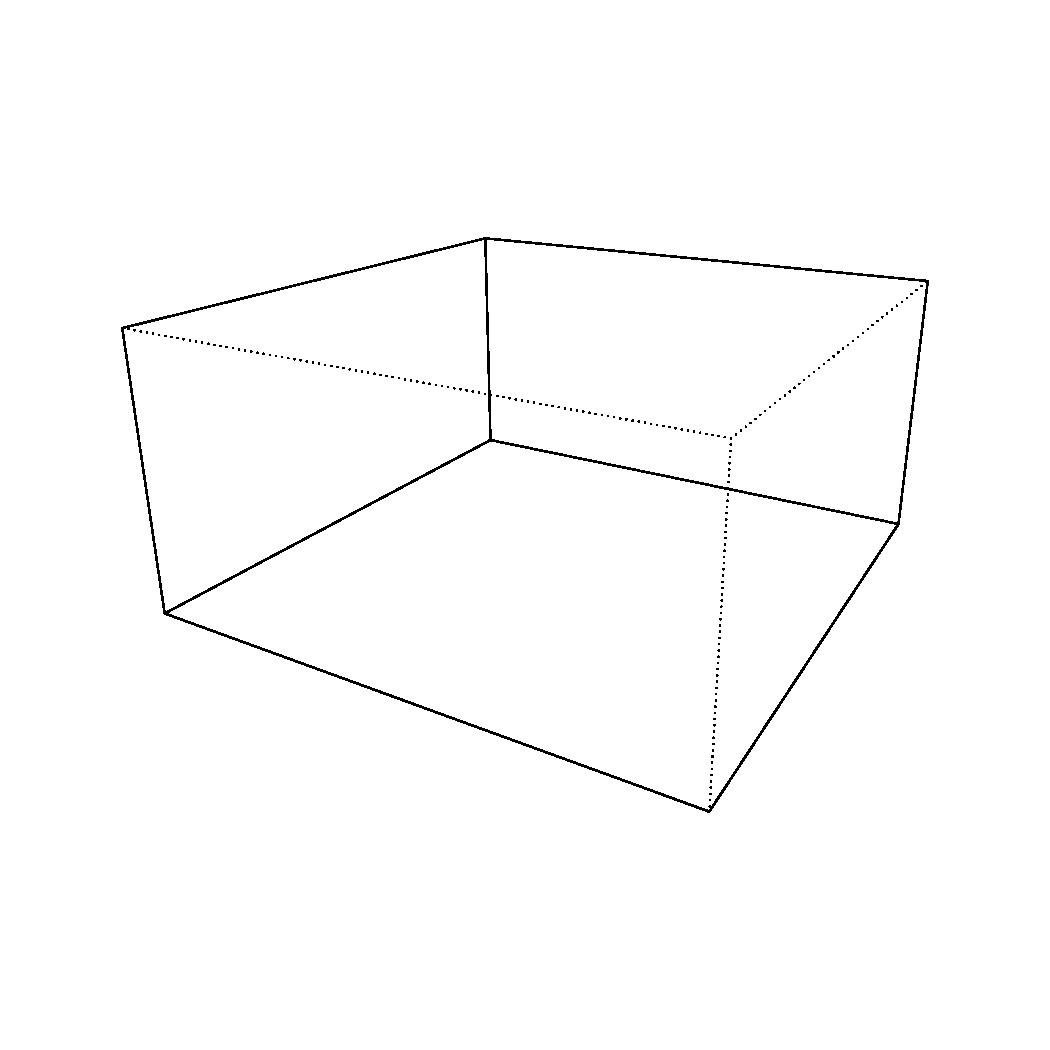
\includegraphics[height = 3.5cm, width = 3.5cm]{figure/axis_example_1.pdf}
  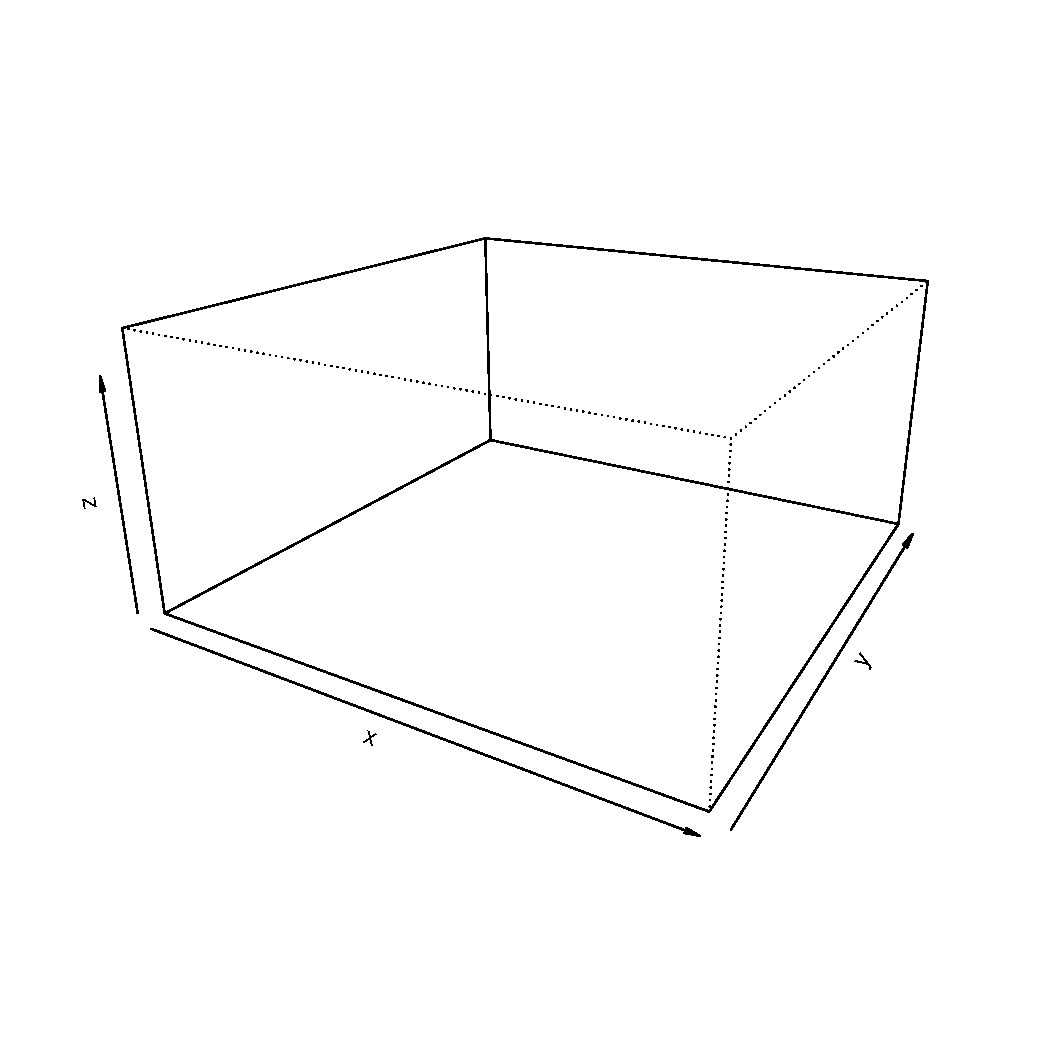
\includegraphics[height = 3.5cm, width = 3.5cm]{figure/axis_example_2.pdf}
  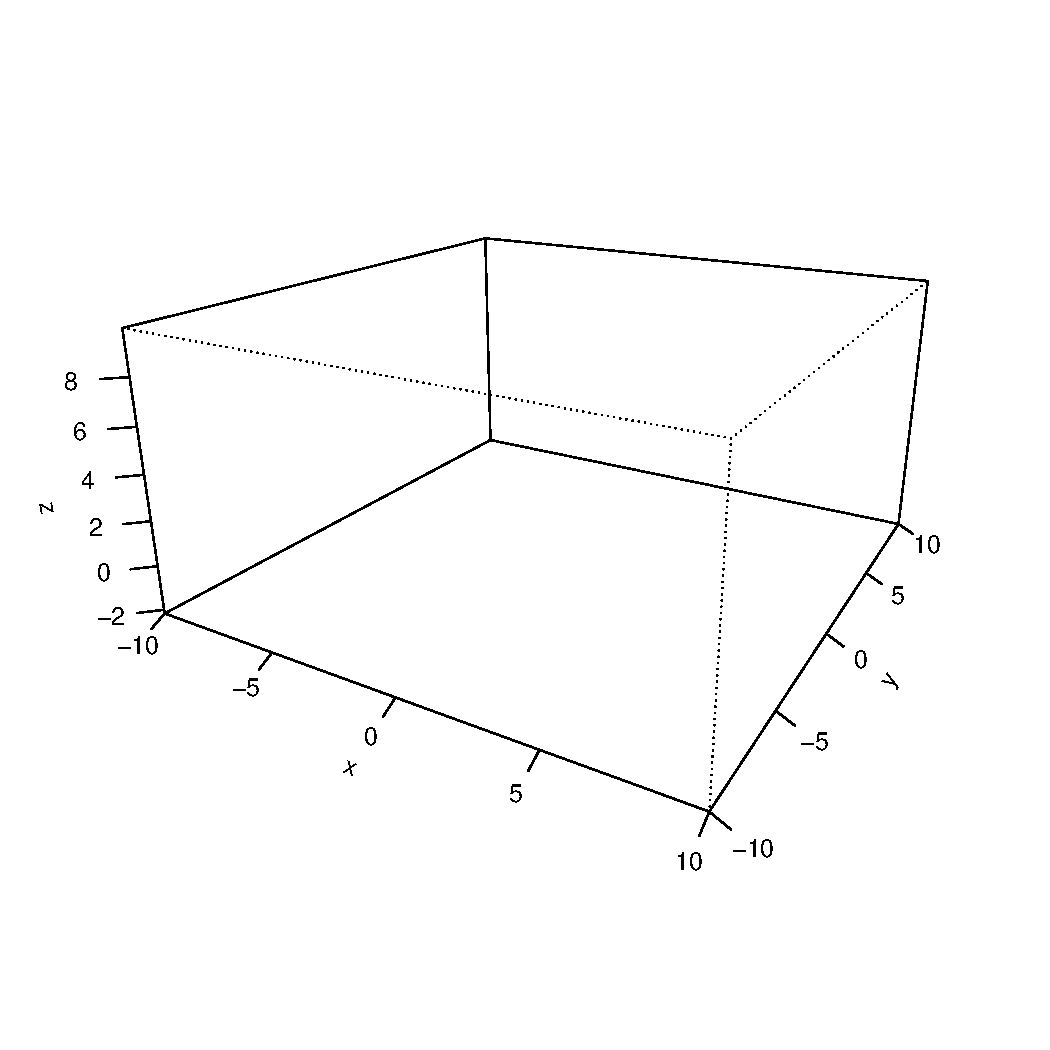
\includegraphics[height = 3.5cm, width = 3.5cm]{figure/axis_example_3.pdf}
  \caption{The Perspective surfaces are been ignored in this example, the left plot shows no axis been drawn, the simple axes been drawn in the middle plot and the right plot shows more detail for each axis.}
  	\label{figure8}
\end{center}
\end{figure}

\section{The Filled Contour Plot}
\subsection{Direct translation from \texttt{C} to \texttt{R}}
The other tasks of this paper is to emulate the Level (Contour) Plots (\texttt{filled.contour}) from \texttt{graphics} to \texttt{grid}. As pervious section, the first step to emulate \texttt{filled.contour} is to access the information from the graphics engine display list. \\

\begin{Schunk}
\begin{Sinput}
> x <- 10*1:nrow(volcano)
> y <- 10*1:ncol(volcano)
> filled.contour(x, y, volcano, color = terrain.colors,
+     plot.title = title(main = "The Topography of Maunga Whau",
+     xlab = "Meters North", ylab = "Meters West"),
+     plot.axes = { axis(1, seq(100, 800, by = 100))
+                   axis(2, seq(100, 600, by = 100)) },
+     key.title = title(main = "Height\n(meters)"),
+     key.axes = axis(4, seq(90, 190, by = 10)))
> xx = recordPlot()
> info = xx[[1]][[12]][[2]]
> head(info[[2]])  ## print the values of x
\end{Sinput}
\begin{Soutput}
[1] 10 20 30 40 50 60
\end{Soutput}
\begin{Sinput}
> head(info[[3]])  ## print the values of y
\end{Sinput}
\begin{Soutput}
[1] 10 20 30 40 50 60
\end{Soutput}
\begin{Sinput}
> dim(info[[4]])  ## print the dimension of z
\end{Sinput}
\begin{Soutput}
[1] 87 61
\end{Soutput}
\begin{Sinput}
> length(info[[5]])  ## print the length of s
\end{Sinput}
\begin{Soutput}
[1] 22
\end{Soutput}
\end{Schunk}


\begin{figure}[h]
\begin{center}
  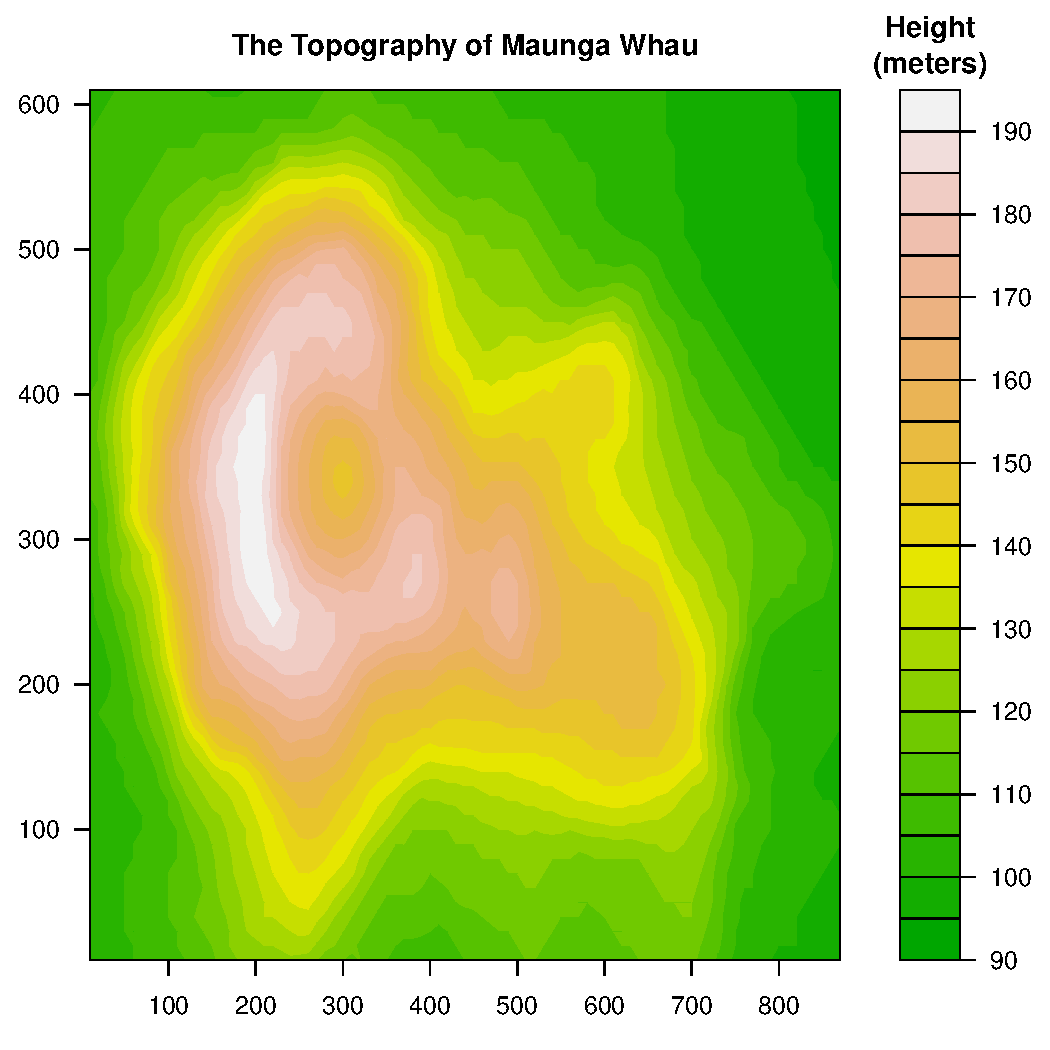
\includegraphics[height = 8cm, width = 8cm]{figure/filled_example_1.pdf}
  \caption{The topography of the Maunga Whau been drawn by using the \texttt{filled.contour}}
  	\label{figure8}
\end{center}
\end{figure}
The example shows the plot of topography of Maunga Whau and also the information from the \texttt{filled.contour} call in the graphics engine display list. Same problem as \texttt{persp()}, there is no way to reproduce this plot directly by only using the coordinates of x, y and z.\\

There is an algorithm to create this contour plot in the \texttt{graphics} package written by \texttt{C}. The first step of the solution will be translated the \texttt{C} code directly to maximize the accuracy.\\

\begin{Schunk}
\begin{Sinput}
> # static void
> # FindPolygonVertices(..., double *x, double *y, double *z, int *npt, ...)
> # {
> #   *npt = 0;
> #   FindCutPoints(low, high, x1,  y1,  z11, x2,  y1,  z21, x, y, z, npt);
> #   FindCutPoints(low, high, y1,  x2,  z21, y2,  x2,  z22, y, x, z, npt);
> #   FindCutPoints(low, high, x2,  y2,  z22, x1,  y2,  z12, x, y, z, npt);
> #   FindCutPoints(low, high, y2,  x1,  z12, y1,  x1,  z11, y, x, z, npt);
> # }
\end{Sinput}
\end{Schunk}
This piece of \texttt{C} code is the algorithm used for calculate the coordinates of the vertex of each polygon in the level contour plot. The parameters $*x$, $*y$, $*z$ are the array pointers which have length of 8 individually, $*npc$ is also a pointer has length of 1. If the \texttt{FindCutPoints} is called, the elements in the arrays of $x$, $y$, $z$ will be modified. In general, we feed the location of memory of $x$, $y$, $z$ and $npt$ to \texttt{FindPolygonVertices()} and modify the values of $x$, $y$, $z$ and $npt$ within the \texttt{FindCutPoints}.\\

For example, the first call of \texttt{FindCutPoints()} modifies the elements in the pointer arrays of $x$, $y$, $z$. The location of elements in arrays been modified will depend on the parameter $*npt$. More specifically, the $*x$ as a function of $x1$ and $x2$, $y$ as a function of $y1$ and so on. The second \texttt{FindCutPoints()} is slightly different, $x$ will depend on a function of $x2$, $y$ as a function of $y1$ and $y2$. In the third \texttt{FindCutPoints()} call, $x$ will depend on a function of $x2$ and $x1$, $y$ will depend on a function of $y2$. Finally, $x$ will depend on a function of $x1$, $y$ depend on the function of $y2$ and $y1$. \\

There is no pointer data structure in \texttt{R} hence we cannot produce the same action as \texttt{C}. One approximation to this action will be as follows:
\begin{Schunk}
\begin{Sinput}
> # lFindPolygonVertices = function(...)
> # {
> #     out = list(); npt = 0
> #     out1 = lFindCutPoints(...)
> #     x = y = z = numeric(8); npt = out1$npt
> #     ...
> #     out$x = out1$x + out2$y + out3$x + out4$y
> #     out$y = out1$y + out2$x + out3$y + out4$x
> #     out$npt = out4$npt
> #     out
> # }
\end{Sinput}
\end{Schunk}
Instead of mortify $x$, $y$, $z$ and $npt$ inside \texttt{FindCutPoints()}, record the values for $x$, $y$, $z$ and $npt$ outside the \texttt{lFindCutPoints()} call in \texttt{R} every time. At last, I combined each individual $x$ and $y$ together as the pervious \texttt{C} code behave. 


\subsection{Vectorization}
...

\chapter{Integrate to \texttt{gridGraphics} package}
\section{Integrate \texttt{persp()}}
\section{Integrate \texttt{filled.contour()}}

\chapter{Testing}
\chapter{Example}
\chapter{Conclusion}
\chapter{Reference}
\chapter{Appendix}
\section{persp.R}
\begin{Schunk}
\begin{Sinput}
> ## initialize and create a viewport prepare for drawing
> perInit = function ( plot, newpage = FALSE, dbox = TRUE ) {
+     info = plot
+     ## [[1]] is the all the grapical information that transfer into grid
+     ## [[3]] is the persp call information
+     ## [[2]] is the plot details eg: x, y, z, xlim, ylim, zlim, col ...
+     ## create a list that store all information from the persp
+     ## then pass the information to per for drawing.
+     ## x is [[2]]; y is [[3]]; z is [[4]]
+     ## xr is [[5]]; yr is [[6]]; zr is [[7]]
+     ## col is [[14]]; border is [[15]]; box is [[19]]
+     ## axes is [[20]], nTicks is [[21]]
+     ## tickType is [[22]]
+     ## xlab/ylab/zlab = [[23]]/[[24]]/[[25]]
+ 	## main is in plot[[1]][[4]][[2]][[2]]
+     ## shade is 0.8, ltheta/lphi = [[16]]/[[17]]
+     ## expand is [[13]], scale is [[12]]
+     out = list(x = info[[2]], y = info[[3]], z = info[[4]],
+                 xr = info[[5]], yr = info[[6]], zr = info[[7]],
+                 col = info[[14]], border = info[[15]][1] ##only allows one color for border
+ 				, dbox = info[[19]],
+                 newpage = newpage, 
+                 phi = info[[9]], theta = info[[8]], r = info[[10]], d = info[[11]],
+                 axes = info[[20]], nTicks = info[[21]], tickType = info[[22]],
+                 xlab = info[[23]], ylab = info[[24]], zlab = info[[25]],
+ 				## parameters in 'par' that need added to per
+                 lwd = info$lwd, lty = info$lty, #col.axis = info$col.axis,
+ 				#col.lab = info$col.lab, 
+ 				cex.lab = info$cex.lab, 
+                 shade = info[[18]], ltheta = info[[16]], lphi = info[[17]],
+                 expand = info[[13]], scale = info[[12]]
+ 				#main = plot[[1]][[4]][[2]][[2]]
+                 )
+     
+     if(out$newpage == TRUE)
+         grid.newpage()
+     out
+ }
> ## main call 
> C_persp = function(plot = NULL, ...)
+ {
+     dev.set(recordDev())
+     par = currentPar(NULL)
+     dev.set(playDev())
+     
+     #information extraction
+     xc = yc = zc = xs = ys = zs = 0
+     plot = perInit(plot, newpage = FALSE)
+     xr = plot$xr; yr = plot$yr; zr = plot$zr
+     xlab = plot$xlab; ylab = plot$ylab; zlab = plot$zlab
+     col.axis = plot$col.axis; col.lab = plot$col.lab; cex.lab = plot$cex.lab
+     nTicks = plot$nTicks; tickType = plot$tickType
+     expand = plot$expand ;scale = plot$scale
+     ltheta = plot$ltheta; lphi = plot$lphi
+     main = plot$main; axes = plot$axes
+     dbox = plot$dbox; shade = plot$shade
+     r = plot$r; d = plot$d; phi = plot$phi; theta = plot$theta
+ 	
+ 	xs = LimitCheck(xr)[1]
+     ys = LimitCheck(yr)[1]
+     zs = LimitCheck(zr)[1]
+     xc = LimitCheck(xr)[2]
+     yc = LimitCheck(yr)[2]
+     zc = LimitCheck(zr)[2]
+ 	
+ 	if(scale == FALSE){
+ 		s = xs
+ 		if(s < ys) s = ys
+ 		if (s < zs) s = zs
+ 		xs = s
+ 		ys = s
+ 		zs = s
+ 	}
+     
+     VT = diag(1, 4)
+     VT = VT %*% Translate(-xc, -yc, -zc)
+     VT = VT %*% Scale(1/xs, 1/ys, expand/zs)
+     VT = VT %*% XRotate(-90.0)
+     VT = VT %*% YRotate(-theta)
+     VT = VT %*% XRotate(phi)
+     VT = VT %*% Translate(0.0, 0.0, -r - d)
+     trans = VT %*% Perspective(d)
+                 
+     border = plot$border[1];
+     if(is.null(plot$lwd)) lwd = 1 else lwd = plot$lwd
+     if(is.null(plot$lty)) lty = 1 else lty = plot$lty
+     if(any(!(is.numeric(xr) & is.numeric(yr) & is.numeric(zr)))) stop("invalid limits")
+     if(any(!(is.finite(xr) & is.finite(yr) & is.finite(zr)))) stop("invalid limits")
+     
+     
+     if(!scale) xs = ys = zs = max(xs, ys, zs)
+     if(is.finite(ltheta) && is.finite(lphi) && is.finite(shade))
+     DoLighting = TRUE else DoLighting = FALSE
+     if (DoLighting) Light = SetUpLight(ltheta, lphi)
+     
+     # create a viewport inside a 'viewport'
+     depth = gotovp(TRUE)
+     lim = PerspWindow(xr, yr, zr, trans, 'r')
+     #vp = viewport(0.5, 0.5, 1, 1, default.units = 'npc',
+     #                xscale = lim[1:2], yscale = lim[3:4])
+     upViewport(depth)
+     
+     incrementWindowAlpha()
+     setWindowPlotAlpha(plotAlpha())
+     setUpUsr(lim)
+     
+ 
+     if (dbox == TRUE) {
+         EdgeDone = rep(0, 12)
+         if(axes == TRUE){
+             depth = gotovp(TRUE)
+             #pushViewport(vp)
+             PerspAxes(xr, yr, zr, ##x, y, z
+                     xlab, ylab, zlab, ## xlab, xenc, ylab, yenc, zlab, zenc
+                     nTicks, tickType, trans, ## nTicks, tickType, VT
+                     lwd, lty, col.axis, col.lab, cex.lab) ## lwd, lty, col.axis, col.lab, cex.lab
+             #upViewport()
+             upViewport(depth)} 
+     } else {
+         EdgeDone = rep(1, 12)
+         xr = yr = zr = c(0,0)
+     }
+     
+     ## draw the behind face first
+     ## return the EdgeDone inorder to not drawing the same Edege two times.
+     depth = gotovp(TRUE)
+     #pushViewport(vp)
+     EdgeDone = PerspBox(0, xr, yr, zr, EdgeDone, trans, 1, lwd)
+     #upViewport()
+     upViewport(depth)
+     
+     depth = gotovp(FALSE)
+     #pushViewport(vp)
+     DrawFacets(plot = plot, z = plot$z, x = plot$x, y = plot$y,     ## basic
+                 xs = 1/xs, ys = 1/ys, zs = expand/zs,               ## Light
+                 col = plot$col, length(plot$col),                   ## cols
+                 ltheta = ltheta, lphi = lphi, Shade = shade, Light = Light, trans = trans)
+     #upViewport()
+     upViewport(depth)
+ 
+     depth = gotovp(TRUE)
+     #pushViewport(vp)
+     EdgeDone = PerspBox(1, xr, yr, zr, EdgeDone, trans, 'dotted', lwd)
+     #upViewport()
+     upViewport(depth)
+     
+     #depth = gotovp(TRUE)
+     #pushViewport(vp)
+ 
+ }
> ####Shade function
> #####################################################################
> LimitCheck = function ( lim ) {
+     ## not finished yet...
+     s = 0.5 * abs(lim[2] - lim[1])
+     c = 0.5 * (lim[2] + lim[1])
+     c(s, c)
+ }
> XRotate = function ( angle ) {
+     TT = diag(1, 4)
+     rad = angle * pi / 180
+     c = cos(rad)
+     s = sin(rad)
+     TT[2, 2] = c;
+     TT[3, 2] = -s;
+     TT[3, 3] = c;
+     TT[2, 3] = s;
+     TT
+ }
> YRotate = function ( angle ) {
+     TT = diag(1, 4)
+     rad = angle * pi / 180
+     c = cos(rad)
+     s = sin(rad)
+     TT[1, 1] = c;
+     TT[3, 1] = s;
+     TT[3, 3] = c;
+     TT[1, 3] = -s;
+     TT
+ }
> ZRotate = function ( angle ) {
+     TT = diag(1, 4)
+     rad = angle * pi / 180
+     c = cos(rad)
+     s = sin(rad)
+     TT[1, 1] = c;
+     TT[2, 1] = -s;
+     TT[2, 2] = c;
+     TT[1, 2] = s;
+     TT
+ }
> Translate = function(x, y, z)
+ {
+     TT = diag(1,4)
+     TT[4, 1] = x
+     TT[4, 2] = y
+     TT[4, 3] = z
+     TT
+ 
+ }
> Scale = function(x, y, z)
+ {
+     TT = diag(1,4)    
+     TT[1, 1] = x
+     TT[2, 2] = y
+     TT[3, 3] = z
+     TT
+ }
> Perspective = function(d)
+ {
+     TT = diag(1,4)
+     TT[3, 4] = -1 / d
+     TT
+ }
> SetUpLight = function ( theta, phi ) {
+     u = c(0, -1, 0, 1)
+     VT = diag(1, 4)
+     VT = VT %*% XRotate(-phi)
+     VT = VT %*% ZRotate(theta)
+     Light = u %*% VT
+ }
> FacetShade = function( u, v, Shade = 0.5, Light ) {
+     nx = u[2] * v[3] - u[3] * v[2]
+     ny = u[3] * v[1] - u[1] * v[3]
+     nz = u[1] * v[2] - u[2] * v[1]
+     sum = sqrt(nx * nx + ny * ny + nz * nz)
+     if (sum == 0) sum = 1
+     nx = nx/sum
+     ny = ny/sum
+     nz = nz/sum
+     sum = 0.5 * (nx * Light[1] + ny * Light[2] + nz * Light[3] + 1)
+     sum^Shade   
+ }
> shadeCol = function( z, x, y, xs, ys, zs, col, ncol = length(col), ltheta, lphi, Shade, Light) {
+     u = v = 0
+     nx = nrow(z)
+     ny = ncol(z)
+     nx1 = nx - 1
+     ny1 = ny - 1
+     cols = 0
+     
+     indx = 0:(length(z))
+     Light = SetUpLight(ltheta, lphi)
+     for(k in 1:(nx1 * ny1)){
+         nv = 0
+         i = (indx[k]) %% nx1 
+         j = (indx[k]) %/% nx1
+         icol = (i + j * nx1) %% ncol + 1
+ 
+         u[1] = xs * (x[i + 2] - x[i + 1])
+ 	    u[2] = ys * (y[j + 1] - y[j + 2])
+ 	    u[3] = zs * (z[(i + 1)+ j * nx + 1] - z[i + (j + 1) * nx + 1])
+ 	    v[1] = xs * (x[i + 2] - x[i + 1])
+ 	    v[2] = ys * (y[j + 2] - y[j + 1])
+ 	    v[3] = zs * (z[(i + 1) + (j + 1) * nx + 1] - z[i + j * nx + 1])
+         icol = (i + j * nx1) %% ncol
+ 	    shade = FacetShade(u, v, Shade = Shade, Light = Light)
+         ##one condiction here..if any bugs then check here...
+         #
+         #
+         shadedCol = col2rgb(col[icol + 1])
+         cols[k] = rgb(shade * shadedCol[1], shade * shadedCol[2], shade * shadedCol[3], maxColorValue = 255)
+     }
+         cols
+ }
> ## shade end...
> #####################################################################
> 
> ## font = 1 -> draw front face
> ## x, y, z are the range of x, y, z-axis
> ## VT = trans
> PerspBox = function(front = 1, x, y, z, EdgeDone, VT, lty, lwd = lwd )
+ {
+     u0 = u1 = u2 = u3 = 0
+     v0 = v1 = v2 = v3 = 0
+     for (f in 1:6) {
+         p0 = Face[f, 1]
+         p1 = Face[f, 2]
+         p2 = Face[f, 3]
+         p3 = Face[f, 4]
+ 
+         u0[1] = x[Vertex[p0, 1]]
+         u0[2] = y[Vertex[p0, 2]]
+         u0[3] = z[Vertex[p0, 3]]
+         u0[4] = 1
+         u1[1] = x[Vertex[p1, 1]]
+         u1[2] = y[Vertex[p1, 2]]
+         u1[3] = z[Vertex[p1, 3]]
+         u1[4] = 1
+         u2[1] = x[Vertex[p2, 1]]
+         u2[2] = y[Vertex[p2, 2]]
+         u2[3] = z[Vertex[p2, 3]]
+         u2[4] = 1
+         u3[1] = x[Vertex[p3, 1]]
+         u3[2] = y[Vertex[p3, 2]]
+         u3[3] = z[Vertex[p3, 3]]
+         u3[4] = 1
+ 
+         v0 = TransVector(u0, VT)
+         v1 = TransVector(u1, VT)
+         v2 = TransVector(u2, VT)
+         v3 = TransVector(u3, VT)
+         
+         v0 = v0/v0[4]
+         v1 = v1/v1[4]
+         v2 = v2/v2[4]
+         v3 = v3/v3[4]
+         
+         d = v1 - v0
+         e = v2 - v1
+         
+         nearby = (d[1]*e[2] - d[2]*e[1]) < 0
+         
+         ## draw the face line by line rather than polygon
+         if ((front && nearby) || (!front && !nearby)) {
+             if (!EdgeDone[Edge[f, 1]]){
+                 grid.lines(c(v0[1], v1[1]), c(v0[2], v1[2]), default.units = 'native',
+                     gp = gpar(lty = lty, lwd = lwd) #vp = 'clipon'
+                     )
+                 EdgeDone[Edge[f, 1]] = EdgeDone[Edge[f, 1]] + 1
+                 }
+             if (!EdgeDone[Edge[f, 2]]){
+                 grid.lines(c(v1[1], v2[1]), c(v1[2], v2[2]), default.units = 'native',
+                     gp = gpar(lty = lty, lwd = lwd) #vp = 'clipon'
+                     )
+                 EdgeDone[Edge[f, 2]] = EdgeDone[Edge[f, 2]] + 1
+                 }
+             if (!EdgeDone[Edge[f, 3]]){
+                 grid.lines(c(v2[1], v3[1]), c(v2[2], v3[2]), default.units = 'native',
+                     gp = gpar(lty = lty, lwd = lwd) #vp = 'clipon'
+                     )
+                 EdgeDone[Edge[f, 3]] = EdgeDone[Edge[f, 3]] + 1
+                 }
+             if (!EdgeDone[Edge[f, 4]]){
+                 grid.lines(c(v3[1], v0[1]), c(v3[2], v0[2]), default.units = 'native',
+                     gp = gpar(lty = lty, lwd = lwd) #vp = 'clipon'
+                     )
+                 EdgeDone[Edge[f, 4]] = EdgeDone[Edge[f, 4]] + 1
+                 }
+         }
+     }
+     EdgeDone
+ }
> dPolygon = function(plot, trans){
+ 
+     x = plot$x; y = plot$y; z = plot$z
+     xr = plot$xr; yr = plot$yr; zr = plot$zr
+     dbox = plot$dbox; lim = plot$lim; mar = plot$mar
+     col = plot$col
+         
+ 
+     ## the total number of polygon that we need to draw	
+ 	nx = length(x)
+ 	ny = length(y)
+     total = nx * ny
+ 	stops = (nx - 1) * (ny - 1)
+ 
+     ## set the temp value for x,y,z prepare for subsetting
+     xTmp = rep(x, length(y))
+     yTmp = rep(y,each = nx)
+     zTmp = as.numeric(z)
+     
+     ## the drawing order is along x-axis, and then along y-axis
+     ## then create a vector like a 4Xn matrix, 
+     ## i.e the first column contain all the first points for every polygons
+     ## the second column contain all the second points for every polygons and so on 
+     pBreak = c(1:total, 1 + 1:total, 1 + nx + 1:total, nx + 1:total)
+     xBreak = xTmp[pBreak]
+     yBreak = yTmp[pBreak]
+     zBreak = zTmp[pBreak]
+     
+     ## draw the box if required
+     ## the vectors now has four paths, every paths contain the information of every points of every polygon
+     ## now we need to change the order of this vector, so that the first four index should be the order for drawing 
+     ## the first points, not the first four points for the first four polygon
+     ## points subsetting 
+     plot.index = rep(
+         c(1, 1 + total, 
+         1 + 2 * total, 
+         1 + 3 * total ),
+         total) + rep(0:(total - 1), each = 4)
+ 
+     ## sequence for 'problem's polygons index, e.g
+     ## along x-axis, there are n-1 polygons, n is the number of points in x direction
+     ## we don't want to draw the nth polygon, hence we deleted those polygon
+     dp = rep((4 * seq(nx,total,nx)), each = 4) - (3:0)
+ 
+     ## final subsetting
+     xCoor = xBreak[c(plot.index)][-dp][1 : (4 * stops)]
+     yCoor = yBreak[c(plot.index)][-dp][1 : (4 * stops)]
+     zCoor = zBreak[c(plot.index)][-dp][1 : (4 * stops)]
+     
+     ## vectorize the cols
+     colRep = rep_len(col, length(xCoor))
+     
+     ## use the first corner of every polygon to determind the order for drawing
+     corn.id = 4* 1:(length(xCoor)/4)
+     xc = xCoor[corn.id]
+     yc = yCoor[corn.id]
+     zc = zCoor[corn.id] 
+     
+     
+     ## method for using the zdepth for changing the drawing order for every polygon
+     orderTemp = cbind(xc, yc, 0, 1) %*% trans 
+     zdepth = orderTemp[, 4]
+ 
+     ## the zdepth of a set of 4 points of each polygon
+     a = order(zdepth, decreasing = TRUE)
+     oo = rep(1:4, length(a)) + rep(a - 1, each = 4) * 4
+ 
+     xyCoor = trans3d(xCoor[oo],
+                     yCoor[oo],
+                     zCoor[oo], trans)
+                     
+     colRep = colRep[a]
+     
+ 
+     ## record the total number of polygon
+     pMax = length(xyCoor$x) / 4
+ 
+     pout = list(xyCoor = xyCoor, pMax = pMax, colRep = colRep, polygonOrder = a)
+     pout
+ }
> DrawFacets = function(plot, z, x, y, xs, ys, zs, col, ncol = length(col), ltheta, lphi, Shade, Light, trans)
+ {
+ 
+     pout = dPolygon(plot, trans)
+     xyCoor = pout$xyCoor
+     pMax = pout$pMax; colRep = pout$colRep
+     polygonOrder = pout$polygonOrder
+     polygons = cbind(xyCoor$x, xyCoor$y)
+     polygon.id = rep(1:pMax, each = 4)
+     
+     if (!is.na(Shade)) {
+         if(is.finite(Shade) && Shade <= 0 ) Shade = 1
+         shadedCol = shadeCol(z, x, y,                       ## x, y, z
+                 xs, ys, zs,                                 ## xs, ys, zs 
+                 plot$col, length(plot$col),                 ## col, ncol
+                 ltheta, lphi, Shade, Light = Light)         ## ltheta, lphi, Shade(not shade)
+         cols = shadedCol[polygonOrder]
+ 
+     } else {
+         cols = rep_len(plot$col, length(polygons[,1]))[polygonOrder]
+     }
+     
+     xrange = range(polygons[,1], na.rm = TRUE)
+     yrange = range(polygons[,2])
+     
+     grid.polygon(polygons[,1], polygons[,2], id = polygon.id,
+                     default.units = 'native', 
+                     gp = gpar(col = plot$border, fill = cols, lty = plot$lty, lwd = plot$lwd))
+ 
+ 
+ }
> ## method for check wheater the axes is front or behind.
> ## return a boxInfo that contain a vector of logical value that tells which face is
> ## front or behind. and a vector of points order as: x1, y1, z1, x2, y2, z2 and so on 
> per.box = function(xlim, ylim, zlim, trans){
+         
+     Near = vector(length = 6)
+     o1 = o2 = o3 = o4 = numeric(0)
+     for (i in 1:6) {
+         p = Face[i, ]
+ 
+         pt = Vertex[p[1], ]
+         u1 = c(xlim[pt[1]] , ylim[pt[2]], zlim[pt[3]], 1)
+ 
+         pt = Vertex[p[2], ]
+         u2 = c(xlim[pt[1]] , ylim[pt[2]], zlim[pt[3]], 1)
+ 
+         pt = Vertex[p[3], ]
+         u3 = c(xlim[pt[1]] , ylim[pt[2]], zlim[pt[3]], 1)
+ 
+         pt = Vertex[p[4], ]
+         u4 = c(xlim[pt[1]] , ylim[pt[2]], zlim[pt[3]], 1)
+ 
+         ## return the points of drawing edges
+         o1 = c(o1,u1[1:3])
+         o2 = c(o2,u2[1:3])
+         o3 = c(o3,u3[1:3])
+         o4 = c(o4,u4[1:3])
+ 
+         v1 = u1 %*% trans
+         v2 = u2 %*% trans
+         v3 = u3 %*% trans
+         v4 = u4 %*% trans
+ 
+         dd = v2/v2[4] - v1/v1[4]
+         ee = v3/v3[4] - v2/v2[4]
+ 
+         Near[i] = (dd[1]*ee[2] - dd[2]*ee[1]) < 0
+     }
+     out = list(Near = Near, O = c(o1, o2, o3, o4))
+     out
+ }
> TransVector = function(u, T) {
+     u %*% T
+ }
> lowest = function (y1, y2, y3, y4) {
+     (y1 <= y2) && (y1 <= y3) && (y1 <= y4)		
+ }
> labelAngle = function(x1, y1, x2, y2){  
+ 
+     dx = abs(x2 - x1)
+     if ( x2 > x1 ) {
+         dy = y2 - y1
+     } else {
+         dy = y1 - y2
+     }
+     
+     if (dx == 0) {
+         if( dy > 0 ) {
+             angle = 90
+         } else {
+             angle = 270
+         }
+     } else {
+         angle = 180/pi * atan2(dy, dx)
+     }
+     angle
+ }	
> PerspAxis = function(x, y, z, axis, axisType, 
+                     nTicks, tickType, label, 
+                     VT, lwd = 1, lty, col.axis = 1,
+                     col.lab = 1, cex.lab = 1){
+ 
+     ## don't know how to use numeric on the switch...
+     axisType = as.character(axisType)
+     tickType = as.character(tickType)
+     u1 = u2 = u3 = c(0.,0.,0.,0.)
+     tickLength = .03
+ 
+     switch(axisType,
+            '1' = {min = x[1]; max = x[2]; range = x},
+            '2' = {min = y[1]; max = y[2]; range = y},
+            '3' = {min = z[1]; max = z[2]; range = z}
+             )
+             
+     d_frac = 0.1 * (max - min)
+     nint = nTicks - 1
+     
+     if(!nint)nint = nint + 1
+     i = nint
+ 
+     ticks = axisTicks(c(min, max), FALSE, nint = nint)
+     min = ticks[1]
+     max = ticks[length(ticks)]
+     nint = length(ticks) - 1
+             
+     ## but maybe not this one... haven't test yet...
+     while((min < range[1] - d_frac || range[2] + d_frac < max) && i < 20) {
+         nint = i + 1
+         ticks = axisTicks(c(min, max), FALSE)
+         range = range(ticks)
+         nint = length(ticks) - 1
+     }
+     
+     ## axp seems working...
+     axp = 0
+     axp[1] = min
+     axp[2] = max
+     axp[3] = nint
+     
+     # Do the following calculations for both ticktypes
+     # Vertex is a 8*3 matrix; i.e. the vertex of a box
+     # AxisStart is a vector of length 8
+     # axis is a output 
+     # u1, u2 are the vectors in 3-d 
+     # the range of x,y,z
+     switch (axisType,
+         '1' = {
+           u1[1] = min
+           u1[2] = y[Vertex[AxisStart[axis], 2]]
+           u1[3] = z[Vertex[AxisStart[axis], 3]]
+         },
+         '2' = {
+           u1[1] = x[Vertex[AxisStart[axis], 1]]
+           u1[2] = min
+           u1[3] = z[Vertex[AxisStart[axis], 3]]
+         },
+         '3' = {
+           u1[1] = x[Vertex[AxisStart[axis], 1]]
+           u1[2] = y[Vertex[AxisStart[axis], 2]]
+           u1[3] = min
+         }
+     )
+     u1[1] = u1[1] + tickLength*(x[2]-x[1])*TickVector[axis, 1]
+     u1[2] = u1[2] + tickLength*(y[2]-y[1])*TickVector[axis, 2]
+     u1[3] = u1[3] + tickLength*(z[2]-z[1])*TickVector[axis, 3]
+     u1[4] = 1
+ 
+     ##axisType, 1 = 'draw x-axis'
+     ##          2 = 'draw y-axis'
+     ##          3 = 'draw z-axis'
+     switch (axisType,
+         '1' = {
+         u2[1] = max
+         u2[2] = u1[2]
+         u2[3] = u1[3]
+         },
+         '2' = {
+         u2[1] = u1[1]
+         u2[2] = max
+         u2[3] = u1[3]
+         },
+         '3' = {
+         u2[1] = u1[1]
+         u2[2] = u1[2]
+         u2[3] = max
+         }
+     )
+     u2[4] = 1
+ 
+     ## ticktype is not working...
+     switch(tickType,
+         '1' = { 
+         u3[1] = u1[1] + tickLength*(x[2]-x[1])*TickVector[axis, 1]
+         u3[2] = u1[2] + tickLength*(y[2]-y[1])*TickVector[axis, 2]
+         u3[3] = u1[3] + tickLength*(z[2]-z[1])*TickVector[axis, 3]
+         },
+         '2' = {
+         u3[1] = u1[1] + 2.5*tickLength*(x[2]-x[1])*TickVector[axis, 1]
+         u3[2] = u1[2] + 2.5*tickLength*(y[2]-y[1])*TickVector[axis, 2]
+         u3[3] = u1[3] + 2.5*tickLength*(z[2]-z[1])*TickVector[axis, 3]
+         }
+     )
+ 
+     ## u3 is the the labels at the center of each axes
+     switch(axisType,
+         '1' = {
+         u3[1] = (min + max)/2
+         },
+         '2' = {
+         u3[2] = (min + max)/2
+         },
+         '3' = {
+         u3[3] = (min + max)/2
+         }
+     )
+ 
+     u3[4] = 1
+ 
+     ## transform the 3-d into 2-d
+     v1 = TransVector(u1, VT)
+     v2 = TransVector(u2, VT)
+     v3 = TransVector(u3, VT)
+ 
+     v1 = v1/v1[4]
+     v2 = v2/v2[4]
+     v3 = v3/v3[4]
+     
+     ## grid set up
+     
+     ## label at center of each axes
+     srt = labelAngle(v1[1], v1[2], v2[1], v2[2])
+     #text(v3[1], v3[2], label, 0.5, srt = srt)
+     grid.text(label = label, x = v3[1], y = v3[2],
+           just = "centre", rot = srt,
+           default.units = "native", #vp = 'clipoff',
+           gp = gpar(col = col.lab, lwd = lwd, cex = cex.lab)
+           )
+     
+     ## tickType is not working.. when = '2'
+     switch(tickType,
+     '1' = {
+     arrow = arrow(angle = 10, length = unit(0.1, "in"),
+                     ends = "last", type = "open")  
+ 	## drawing the tick..
+     
+     grid.lines(x = c(v1[1], v2[1]), y = c(v1[2], v2[2]),
+           default.units = "native", arrow = arrow, #vp = 'clipoff',
+           gp = gpar(col = 1, lwd = lwd , lty = lty )
+           )
+        },
+     ## '2' seems working
+     '2' = {
+         at = axisTicks(range, FALSE, axp, nint = nint)
+         for(i in 1:length(at)){
+             switch(axisType, 
+                 '1' = {
+                 u1[1] = at[i]
+                 u1[2] = y[Vertex[AxisStart[axis], 2]]
+                 u1[3] = z[Vertex[AxisStart[axis], 3]]
+                 },
+                 '2' = {
+                 u1[1] = x[Vertex[AxisStart[axis], 1]]
+                 u1[2] = at[i]
+                 u1[3] = z[Vertex[AxisStart[axis], 3]]
+                 },
+                 '3' = {
+                 u1[1] = x[Vertex[AxisStart[axis], 1]]
+                 u1[2] = y[Vertex[AxisStart[axis], 2]]
+                 u1[3] = at[i]
+                 }
+             )
+             
+             tickLength = 0.03
+             
+             u1[4] = 1
+             u2[1] = u1[1] + tickLength*(x[2]-x[1])*TickVector[axis, 1]
+             u2[2] = u1[2] + tickLength*(y[2]-y[1])*TickVector[axis, 2]
+             u2[3] = u1[3] + tickLength*(z[2]-z[1])*TickVector[axis, 3]
+             u2[4] = 1
+             u3[1] = u2[1] + tickLength*(x[2]-x[1])*TickVector[axis, 1]
+             u3[2] = u2[2] + tickLength*(y[2]-y[1])*TickVector[axis, 2]
+             u3[3] = u2[3] + tickLength*(z[2]-z[1])*TickVector[axis, 3]
+             u3[4] = 1
+             v1 = TransVector(u1, VT)
+             v2 = TransVector(u2, VT)
+             v3 = TransVector(u3, VT)
+                         
+             v1 = v1/v1[4]
+             v2 = v2/v2[4]
+             v3 = v3/v3[4]
+             
+             ## Draw tick line
+             grid.lines(x = c(v1[1], v2[1]), y = c(v1[2], v2[2]),
+                 default.units = "native", ##vp = 'clipoff',
+                 gp = gpar(col = col.axis, lwd = lwd, lty = lty)
+                 )
+ 
+             ## Draw tick label
+             lab = at[i]
+             #text(v3[1], v3[2], label, 0.5, srt = srt)
+             grid.text(label = lab, x = v3[1], y = v3[2],
+                   just = "centre",
+                   default.units = "native", #vp = 'clipoff',
+                   gp = gpar(col = col.axis, adj = 1, pos = 0.5, cex = 1)
+                   )
+             }
+         }
+     )
+ }
> PerspAxes = function(x, y, z, 
+                     xlab, 
+                     ylab, 
+                     zlab, 
+                     nTicks, tickType, VT, 
+ 					## parameters in par
+                     lwd = 1, lty = 1, col.axis = 1, col.lab = 1, cex.lab = 1)
+ {
+     xAxis = yAxis = zAxis = 0 ## -Wall 
+     u0 = u1 = u2 = u3 = 0
+ 
+     u0[1] = x[1]; u0[2] = y[1]; u0[3] = z[1]; u0[4] = 1
+     u1[1] = x[2]; u1[2] = y[1]; u1[3] = z[1]; u1[4] = 1
+     u2[1] = x[1]; u2[2] = y[2]; u2[3] = z[1]; u2[4] = 1
+     u3[1] = x[2]; u3[2] = y[2]; u3[3] = z[1]; u3[4] = 1
+ 
+     v0 = TransVector(u0, VT)
+     v1 = TransVector(u1, VT)
+     v2 = TransVector(u2, VT)
+     v3 = TransVector(u3, VT)
+ 
+     v0 = v0/v0[4]
+     v1 = v1/v1[4]
+     v2 = v2/v2[4]
+     v3 = v3/v3[4]
+ 
+     if (lowest(v0[2], v1[2], v2[2], v3[2])) {
+         xAxis = 1
+         yAxis = 2
+     } else if (lowest(v1[2], v0[2], v2[2], v3[2])) {
+         xAxis = 1
+         yAxis = 4
+     } else if (lowest(v2[2], v1[2], v0[2], v3[2])) {
+         xAxis = 3
+         yAxis = 2
+     } else if (lowest(v3[2], v1[2], v2[2], v0[2])) {
+         xAxis = 3
+         yAxis = 4
+     } else
+         warning("Axis orientation not calculated")
+     ## drawing x and y axes
+     
+     PerspAxis(x, y, z, xAxis, '1', nTicks, tickType, xlab, VT, lwd = lwd, lty = lty, col.axis = col.axis, col.lab = col.lab, cex.lab = cex.lab)
+     PerspAxis(x, y, z, yAxis, '2', nTicks, tickType, ylab, VT, lwd = lwd, lty = lty, col.axis = col.axis, col.lab = col.lab, cex.lab = cex.lab)
+ 
+     ## Figure out which Z axis to draw
+     if (lowest(v0[1], v1[1], v2[1], v3[1])) {
+             zAxis = 5
+         }else if (lowest(v1[1], v0[1], v2[1], v3[1])) {
+             zAxis = 6
+         }else if (lowest(v2[1], v1[1], v0[1], v3[1])) {
+             zAxis = 7
+         }else if (lowest(v3[1], v1[1], v2[1], v0[1])) {
+             zAxis = 8
+         }else
+     warning("Axis orientation not calculated")
+ 
+     ## drawing the z-axis
+     PerspAxis(x, y, z, zAxis, '3', nTicks, tickType, zlab, VT, lwd = lwd, lty = lty, col.axis = col.axis, col.lab = col.lab, cex.lab = cex.lab)
+ }
> PerspWindow = function(xlim, ylim, zlim, VT, style)
+ {
+     xmax = xmin = ymax = ymin = u = 0
+     u[4] = 1
+     for (i in 1:2) {
+         u[1] = xlim[i]
+         for (j in 1:2) {
+             u[2] = ylim[j]
+             for (k in 1:2) {
+                 u[3] = zlim[k]
+                 v = TransVector(u, VT)
+                 xx = v[1] / v[4]
+                 yy = v[2] / v[4]
+                 if (xx > xmax) xmax = xx
+                 if (xx < xmin) xmin = xx
+                 if (yy > ymax) ymax = yy
+                 if (yy < ymin) ymin = yy
+           }
+         }
+     }
+     pin1 = convertX(unit(1.0, 'npc'), 'inches', valueOnly = TRUE)
+     pin2 = convertY(unit(1.0, 'npc'), 'inches', valueOnly = TRUE)
+     xdelta = abs(xmax - xmin)
+     ydelta = abs(ymax - ymin)
+     xscale = pin1 / xdelta
+     yscale = pin2 / ydelta
+     scale = if(xscale < yscale) xscale else yscale
+     xadd = .5 * (pin1 / scale - xdelta);
+     yadd = .5 * (pin2 / scale - ydelta);
+     ## GScale in C
+     xrange = GScale(xmin - xadd, xmax + xadd, style)
+     yrange = GScale(ymin - yadd, ymax + yadd, style)
+     c(xrange, yrange)
+   
+ }
> GScale = function(min, max, style)
+ {
+   switch(style, 
+          'r' = {temp = 0.04 * (max - min)
+          min = min - temp
+          max = max + temp
+          },
+          'i' = {}
+   )
+   c(min, max)
+ }
> ## global variables.
> TickVector = matrix(ncol = 3, byrow = TRUE, data = c(
+     0, -1, -1,
+     -1, 0, -1,
+     0, 1, -1,
+     1, 0, -1,
+     -1, -1, 0,
+     1, -1, 0,
+     -1, 1, 0,
+     1, 1, 0 ))
> Vertex = matrix(ncol = 3, byrow = TRUE, data = c(
+ 	1, 1, 1,  #xlim[1], ylim[1], zlim[1]
+ 	1, 1, 2,  #xlim[1], ylim[1], zlim[2]
+ 	1, 2, 1,
+ 	1, 2, 2,
+ 	2, 1, 1,
+ 	2, 1, 2,
+ 	2, 2, 1,
+ 	2, 2, 2 ))
> Face  = matrix (ncol = 4, byrow = TRUE, data = c(
+     1, 2, 6, 5,
+     3, 7, 8, 4,
+     1, 3, 4, 2,
+     5, 6, 8, 7,
+     1, 5, 7, 3,
+     2, 4, 8, 6 ))
> Edge  = matrix (ncol = 4, byrow = TRUE, data = c(
+     0, 1, 2, 3,
+     4, 5, 6, 7,
+     8, 7, 9, 0,
+     2,10, 5,11,
+     3,11, 4, 8,
+     9, 6,10, 1)) + 1
> AxisStart = c(1, 1, 3, 5, 1, 5, 3, 7)
> 
> 
> 
\end{Sinput}
\end{Schunk}
\newpage
\section{filled.contour.R}
\begin{Schunk}
\begin{Sinput}
> lFindPolygonVertices = function(low,  high,
+ 		     x1,  x2,  y1,  y2,
+ 		     z11,  z21,  z12,  z22,
+ 		     x,  y,  z, npt, iii)
+ {
+     out = list(); npt = 0
+     #      FindCutPoints(low, high, x1,  y1,  z1,  x2,  y2,  z2,  x, y, z, npt)
+     out1 = lFindCutPoints(low, high, x1,  y1,  z11, x2,  y1,  z21, x, y, z, npt)
+     x = y = z = numeric(8); npt = out1$npt
+     out2 = lFindCutPoints(low, high, y1,  x2,  z21, y2,  x2,  z22, y, x, z, npt)
+     x = y = z = numeric(8); npt = out2$npt
+     out3 = lFindCutPoints(low, high, x2,  y2,  z22, x1,  y2,  z12, x, y, z, npt)
+     x = y = z = numeric(8); npt = out3$npt
+     out4 = lFindCutPoints(low, high, y2,  x1,  z12, y1,  x1,  z11, y, x, z, npt)
+ 
+     out$x = out1$x + out2$y + out3$x + out4$y
+     out$y = out1$y + out2$x + out3$y + out4$x
+     out$npt = out4$npt
+     out
+ }
> lC_filledcontour = function(plot)
+ {
+     dev.set(recordDev())
+     par = currentPar(NULL)
+     dev.set(playDev())
+ 
+     x  =  plot[[2]]
+     y = plot[[3]]
+     z = plot[[4]]
+     sc = plot[[5]]
+     px = py = pz = numeric(8)
+     scol = plot[[6]]
+ 
+     nx = length(x)
+     ny = length(y)
+     if (nx < 2 || ny < 2) stop("insufficient 'x' or 'y' values")
+ 
+     ## do it this way as coerceVector can lose dims, e.g. for a list matrix
+     if (nrow(z) != nx || ncol(z) != ny) stop("dimension mismatch")
+ 
+     nc = length(sc)
+     if (nc < 1) warning("no contour values")
+ 
+     ncol = length(scol)
+     
+     # debug
+     # ii = 0; iii = 0 ## a = 0
+     
+     depth = gotovp(TRUE)
+     for(i in 1:(nx - 1)){
+     for(j in 1:(ny - 1)){
+         for(k in 1:(nc - 1)){
+             npt = 0
+             #iii = iii + 1
+             out = lFindPolygonVertices(sc[k], sc[k + 1],
+                     x[i], x[i + 1],
+                     y[j], y[j + 1],
+                     z[i + (j - 1) * nx],
+                     z[i + 1 + (j - 1) * nx],
+                     z[i + (j) * nx],
+                     z[i + 1 + (j) * nx],
+                     px, py, pz, npt)
+             
+             npt = out$npt
+             
+             ## debug
+             # ii = ii + 1
+             # if(ii <= 1000 & npt > 2) {print(out$x)}
+             if(npt > 2)
+             { 
+                 #ii = ii + 1
+                 #a[ii] = npt
+                 # print(ii)
+                 
+                 #if(ii >= 1 && ii <= 5 ) {
+                  #   print(out$x); 
+                  #   print(paste('#of polygons: ', iii)); 
+                 #    print(paste('npt: ', out$npt))}
+                 
+                 grid.polygon(out$x[1:npt], out$y[1:npt], default.units = 'native',
+                     gp = gpar(fill = scol[(k - 1) %% ncol + 1], col = NA))
+             }
+         }
+     }
+     }
+     upViewport(depth)
+    
+ }
> lFindCutPoints = function( low,  high,
+ 	       x1,  y1,  z1,
+ 	       x2,  y2,  z2,
+ 	       x,  y,  z,
+ 	       npt)
+ {
+     x = y = z = numeric(8)
+     if (z1 > z2 ) {
+         if (z2 > high || z1 < low){
+             return(out = list(x = x, y = y, z = z, npt = npt))
+         }
+ 
+         if (z1 < high) {
+             x[npt + 1] = x1
+             y[npt + 1] = y1
+             z[npt + 1] = z1
+             npt = npt + 1
+         } else if (z1 == Inf) {
+             x[npt + 1] = x2
+             y[npt + 1] = y1
+             z[npt + 1] = z2
+             npt = npt + 1
+         } else {
+             c = (z1 - high) / (z1 - z2)
+             x[npt + 1] = x1 + c * (x2 - x1)
+             y[npt + 1] = y1
+             z[npt + 1] = z1 + c * (z2 - z1)
+             npt = npt + 1
+         }
+         
+         if (z2 == -Inf) {
+             x[npt + 1] = x1
+             y[npt + 1] = y1
+             z[npt + 1] = z1
+             npt = npt + 1
+         } else if (z2 <= low) {
+             c = (z2 -low) / (z2 - z1)
+             x[npt + 1] = x2 - c * (x2 - x1)
+             y[npt + 1] = y1
+             z[npt + 1] = z2 - c * (z2 - z1)
+             npt = npt + 1
+         }
+         
+     } else if (z1 < z2) {
+         if (z2 < low || z1 > high) {
+                 return(out = list(x = x, y = y, z = z, npt = npt))
+         }
+         
+         if (z1 > low) {
+             x[npt + 1] = x1
+             y[npt + 1] = y1
+             z[npt + 1] = z1
+             npt = npt + 1
+         } else if (z1 == -Inf) {
+             x[npt + 1] = x2
+             y[npt + 1] = y1
+             z[npt + 1] = z2
+             npt = npt + 1
+         } else { 
+             c = (z1 - low) / (z1 - z2)
+             x[npt + 1] = x1 + c * (x2 - x1)
+             y[npt + 1] = y1
+                 z[npt + 1] = z1 + c * (z2 - z1)
+             npt = npt + 1
+         }
+         
+         if (z2 < high) {
+         } else if (z2 == Inf) {
+             x[npt + 1] = x1
+             y[npt + 1] = y1
+             z[npt + 1] = z1
+             npt = npt + 1
+         } else {
+             c = (z2 - high) / (z2 - z1)
+             x[npt + 1] = x2 - c * (x2 - x1)
+             y[npt + 1] = y1
+             z[npt + 1] = z2 - c * (z2 - z1)
+             npt = npt + 1
+         }
+     } else {
+         if(low <= z1 && z1 <= high) {
+             x[npt + 1] = x1
+             y[npt + 1] = y1
+             z[npt + 1] = z1
+             npt = npt + 1
+         }
+     }
+     out = list(x = x, y = y, z = z, npt = npt)
+     out
+ }
> ## vectorization version
> FindPolygonVertices = function(low,  high,
+ 		     x1,  x2,  y1,  y2,
+ 		     z11,  z21,  z12,  z22,
+              colrep){
+ 
+     v1 = FindCutPoints(low, high, x1, y1, x2, y1, z11, z21)
+     v2 = FindCutPoints(low, high, y1, x2, y2, x2, z21, z22)
+     v3 = FindCutPoints(low, high, x2, y2, x1, y2, z22, z12)
+     v4 = FindCutPoints(low, high, y2, x1, y1, x1, z12, z11)
+ 
+     vx = cbind(v1[[1]], v2[[2]], v3[[1]], v4[[2]])
+     vy = cbind(v1[[2]], v2[[1]], v3[[2]], v4[[1]])
+     
+     ##  track the coordinate for x and y( if non-NA's)
+     index = rowSums(!is.na(vx) )
+     ## keep if non-NAs row >= 2 (npt >= 2)
+     vx = t(vx)
+     vy = t(vy)
+     xcoor.na = as.vector(vx[, index > 2])
+     ycoor.na = as.vector(vy[, index > 2])
+     ## delete all NA's,
+     xcoor = xcoor.na[!is.na(xcoor.na)]
+     ycoor = ycoor.na[!is.na(ycoor.na)]
+ 
+     id.length = index[index > 2]
+     cols = colrep[index > 2]
+     
+     out = list(x = xcoor, y = ycoor, id.length = id.length, cols = cols)
+     outs = out
+     out
+ }
> C_filledcontour = function(plot)
+ {
+     dev.set(recordDev())
+     par = currentPar(NULL)
+     dev.set(playDev())
+ 
+     x = plot[[2]]
+     y = plot[[3]]
+     z = plot[[4]]
+     s = plot[[5]]
+     cols = plot[[6]]
+     
+     ns = length(s)
+     nx = length(x)
+     ny = length(y)
+ 
+     x1 = rep(x[-nx], each = ny - 1)
+     x2 = rep(x[-1], each = ny - 1)
+     y1 = rep(y[-ny], nx - 1)
+     y2 = rep(y[-1], nx - 1)
+ 
+     z11 = as.numeric(t(z[-nx, -ny]))
+     z21 = as.numeric(t(z[-1, -ny ]))
+     z12 = as.numeric(t(z[-nx, -1]))
+     z22 = as.numeric(t(z[-1, -1]))
+     
+     x1 = rep(x1, each = ns - 1)
+     x2 = rep(x2, each = ns - 1)
+     y1 = rep(y1, each = ns - 1)
+     y2 = rep(y2, each = ns - 1)
+     z11 = rep(z11, each = ns - 1)
+     z12 = rep(z12, each = ns - 1)
+     z21 = rep(z21, each = ns - 1)
+     z22 = rep(z22, each = ns - 1)
+     low = rep(s[-ns], (nx - 1) * (ny - 1))
+     high = rep(s[-1], (nx - 1) * (ny - 1))
+     
+     ## rep color until the same length of x, then subsetting 
+     colrep = rep(cols, nx * ny)
+     
+     ## feed color as well as subseeting as x and y
+     out = FindPolygonVertices(
+                 low = low, high = high,
+                 x1 = x1, x2 = x2, 
+                 y1 = y1, y2 = y2,
+                 z11 = z11, z21 = z21, 
+                 z12 = z12, z22 = z22, colrep = colrep)
+     ## actual drawing
+     depth = gotovp(TRUE)
+     grid.polygon(out$x, out$y, default.units = 'native', id.lengths = out$id.length,
+              gp = gpar(fill = out$cols, col = NA))
+     upViewport(depth)
+ }
> FindCutPoints = function(low, high, x1, y1, x2, y2, z1, z2)
+ {
+ ## inner condiction begin
+     ## first ocndiction
+     c = (z1 - high) / (z1 - z2)
+     cond1 = z1 < high
+     cond2 = z1 == Inf
+     cond3 = z2 > high | z1 < low
+     
+     x.1 = ifelse(cond1, x1, 
+               ifelse(cond2, x2, x1 + c * (x2 - x1)))
+     x.1 = ifelse(cond3, NA, x.1)
+                 
+     y.1 = ifelse(cond1, y1, 
+                ifelse(cond2, y1, y1))
+     y.1 = ifelse(cond3, NA, y.1)
+     
+     cond4 = z2 == -Inf
+     cond5 = z2 <= low
+     cond6 = z2 > high | z1 < low
+ 
+     c = (z2 -low) / (z2 - z1)
+     x.2 = ifelse(cond4, x1,
+              ifelse(cond5, x2 - c * (x2 - x1), NA))
+     x.2 = ifelse(cond6, NA, x.2)
+              
+     y.2 = ifelse(cond4, y1,
+               ifelse(cond5, y1, NA))
+     y.2 = ifelse(cond6, NA, y.2)
+ 
+     ## second condiction
+     cond7 = z1 > low
+     cond8 = z1 == -Inf
+     cond9 = z2 < low | z1 > high
+     
+     c = (z1 - low) / (z1 - z2)
+     x_1 = ifelse(cond7, x1, 
+                 ifelse(cond8, x2, x1 + c * (x2 - x1)))
+     x_1 = ifelse(cond9, NA, x_1)
+                 
+     y_1 = ifelse(cond7, y1, 
+                 ifelse(cond8, y1, y1))
+     y_1 = ifelse(cond9, NA, y_1)
+     
+     cond10 = z2 < high
+     cond11 = z2 == Inf
+     cond12 = z2 < low | z1 > high
+                 
+     c = (z2 - high) / (z2 - z1)
+     x_2 = ifelse(cond10, NA, 
+                 ifelse(cond11, x1, x2 - c * (x2 - x1)))
+     x_2 = ifelse(cond12, NA, x_2)
+                 
+     y_2 = ifelse(cond10, NA, 
+                 ifelse(cond11, y1, y1))
+     y_2 = ifelse(cond12, NA, y_2)
+                 
+     ## third condiction
+     cond13 = low <= z1 & z1 <= high
+     x..1 = ifelse(cond13, x1, NA)
+     y..1 = ifelse(cond13, y1, NA)
+ ## inner condiction end
+     
+ ## outer condiction 
+     cond14 = z1 > z2
+     cond15 = z1 < z2
+ 
+     xout.1 = ifelse(cond14, x.1,
+                 ifelse(cond15, x_1,
+                         x..1))
+     xout.2 = ifelse(cond14, x.2,
+                 ifelse(cond15, x_2,
+                         NA))						
+ 
+     yout.1 = ifelse(cond14, y.1,
+                 ifelse(cond15, y_1,
+                         y..1))
+     yout.2 = ifelse(cond14, y.2,
+                 ifelse(cond15, y_2,
+                         NA))			
+ ## outer condiction end
+ 
+     ## return x1, x2, y1, y2
+     xout = cbind(xout.1, xout.2)
+     yout = cbind(yout.1, yout.2)
+     list(xout, yout)
+ }
\end{Sinput}
\end{Schunk}
\end{document}
